\chapter{Appendix for Chapter 3}

\section{Transformation Theory}\label{Appendix: theorem 3}
\begin{theorem} \label{Theorem: transformation of normalization}
Consider a linear transformation $x=\sigma \xi + \mu$. If a function $f(x)$ defined on $\mathbb{R}$ satisfies the conditions of Theorem~\ref{Theorem: Stenger} for some positive constants $d$, $\alpha$, and $\beta$, specifically:

(1) $f$ is an element of the Hardy space $H^1(\mathcal{D}_d)$, where $\mathcal{D}_d=\{z\in \mathbb{C} \mid |\Im z|<d\}$;

(2) $f$ exhibits exponential decay on the real line, satisfying $|f(x)| \leq \alpha \exp (-\beta|x|)$ for all $x \in \mathbb{R}$;

then the transformed function $\tilde{f}(\xi)=f(\sigma\xi+\mu)$ defined on $\mathbb{R}$ satisfies conditions (1) and (2) for some positive constants $\tilde{\alpha}$, $\tilde{\beta}$, and $\tilde{d}$.
\end{theorem}

\begin{proof}
To establish condition (1), we observe that since $\mu$ and $\sigma$ are real numbers, the following equivalences hold:
\begin{equation}
f(x)\in H^1(\mathcal{D}_d)        
\end{equation}
$\Leftrightarrow$
\begin{equation}
    \lim_{\varepsilon \rightarrow 0} \int_{\partial \mathcal{D}_d(\varepsilon)}|f(z)||\mathrm{d} z|<\infty
\end{equation}
$\Leftrightarrow$
\begin{equation}
   \int_{-\infty}^{\infty}|f(x \pm id)|\mathrm{d} x<\infty 
\end{equation}

Consequently:
\begin{equation}
\begin{aligned}
         &\int_{-\infty}^{\infty}|\tilde{f}(\tilde{x}\pm i\tilde{d})|\mathrm{d} \tilde{x}\\
         = & \int_{-\infty}^{\infty}|f(\sigma \tilde{x}+\mu \pm i\sigma \tilde{d})|\mathrm{d} x \\
         = & \int_{-\infty}^{\infty}|f(x^\prime \pm id^\prime)|\mathrm{d} x^\prime, \text{ where } x^\prime=\sigma \tilde{x} +\mu,d^\prime = \sigma \tilde{d} 
\end{aligned}
\end{equation}

For $d^\prime < d$, equivalently $\tilde{d}<\frac{d}{\sigma}$, we have $ \int_{-\infty}^{\infty}|f(x^\prime\pm id^\prime)|\mathrm{d} x^\prime < \infty$, which implies $\tilde{f}(\xi)\in H^1(\mathcal{D}_{\tilde{d}})$. Since $\frac{d}{\sigma}>0$, the existence of $\tilde{d}$ is established, satisfying condition (1).

For condition (2), given that $|\tilde{f}(\xi)| \leq \alpha \exp (-\beta|\sigma\xi+\mu|)$ for all $\xi \in \mathbb{R}$, we seek positive constants $\tilde{\alpha}$ and $\tilde{\beta}$ satisfying:
\begin{equation}
     \alpha \exp (-\beta|\sigma\xi+\mu|) \leq \tilde{\alpha}\exp (-\tilde{\beta}|\xi|)
\end{equation}

This inequality can be expressed logarithmically as:
\begin{equation}
    \log \alpha -\beta|\sigma\xi+\mu| \leq \log \tilde{\alpha} -\tilde{\beta}|\xi| 
\end{equation}
which yields:
\begin{equation}
    \tilde{\beta} \leq \frac{\log \frac{\tilde{\alpha}}{\alpha}}{|\xi|}+\beta\left|\sigma+\frac{\mu}{\xi}\right|, \text{ for } \xi\neq 0.
\end{equation}

For $\tilde{\alpha}>\alpha$, there exists a positive $\tilde{\beta}$ satisfying this inequality. When $\xi=0$, we observe that $\alpha \exp (-\beta|\sigma\xi+\mu|) \leq \alpha < \tilde{\alpha}$. Therefore, appropriate values of $\tilde{\alpha}$ and $\tilde{\beta}$ exist.

Combining these results, we have demonstrated the existence of positive constants $\tilde{d}$, $\tilde{\alpha}$, and $\tilde{\beta}$ such that $\tilde{f}$ satisfies both conditions (1) and (2).
\end{proof}

\section{Function Specifications}\label{Appendix: details of approximate functions}
This section provides explicit expressions for the functions utilized in Tables~\ref{table: function approxmation} and \ref{table: function approxmation rest}.

\begin{enumerate}
    \item Low-frequency sinusoidal function (\textit{sin-low}):
    \begin{equation}
        f(x) = \sin (4\pi x),\quad x\in [-1,1]
    \end{equation}
    
    \item High-frequency sinusoidal function (\textit{sin-high}):
    \begin{equation}
        f(x) = \sin (400\pi x),\quad x\in [-1,1]
    \end{equation}
    
    \item Boundary layer function (\textit{bl}):
    \begin{equation}
        f(x) = e^{-100x},\quad x\in [0,1]
    \end{equation}
    
    \item Square root function (\textit{sqrt}):
    \begin{equation}
        f(x) = \sqrt{x},\quad x\in [0,1]
    \end{equation}
    
    \item Double exponential function (\textit{double-exponential}):
    \begin{equation}
        f(x)=\frac{x(1-x) \mathrm{e}^{-x}}{(1 / 2)^2+(x-1 / 2)^2}, \quad x \in[0,1]
    \end{equation}
    
    \item Multiple square root function (\textit{multi-sqrt}):
    \begin{equation}
        f(x) = x^{1/2}(1-x)^{3/4},\quad x\in [0,1]
    \end{equation}
    
    \item Piecewise function (\textit{piece-wise}):
    \begin{equation}
        f(x)=\left\{
        \begin{aligned}
         & \sin(20 \pi x) + x^2,&\quad x\in [0,0.5] \\
         & 0.5x e^{-x} + |\sin(5\pi x)|,&\quad x\in [0.5,1.5] \\
         & \log (x - 1) / \log(2) - \cos(2  \pi x),&\quad x\in [1.5,2]
        \end{aligned}
        \right.
    \end{equation}
    
    \item Spectral bias function (\textit{spectral-bias}):
    \begin{equation}
        f(x)=\left\{
        \begin{aligned}
         & \sum_{k=1}^4\sin(k x) + 5,&\quad x\in [-1, 0] \\
         & \cos(10x),&\quad x\in [0, 1] \\
        \end{aligned}
        \right.
    \end{equation}

    \item Two-dimensional multimodal function 1 (\textit{multimodal1-2d}):
    \begin{equation}
        f(\boldsymbol{x})=-|\sin(x_1) \cdot \cos(x_2)| \cdot \exp \left(|1-\frac{\sqrt{x_1^2+x_2^2}}{\pi}|\right),\quad \boldsymbol{x}\in [0,1]^{2}
    \end{equation}
    
    \item Two-dimensional multimodal function 2 (\textit{multimodal2-2d}):
    \begin{equation}
    \begin{aligned}
        f(\boldsymbol{x}) = & -20 e^{-0.2 \sqrt{x_1^2+x_2^2}}-e^{\cos(2\pi x_1) +\cos(2\pi x_2)}\\
        &+e+20,\quad \boldsymbol{x}\in [-1,1]^{2}
    \end{aligned}
    \end{equation}
    
    \item Two-dimensional fractal function (\textit{fractal-2d}):
    \begin{equation}
    \begin{aligned}
        f(\boldsymbol{x})= & [\sin(10\pi x_1) \cos(10\pi x_2)+\sin(\pi(x_1^2+x_2^2))+|x_1-x_2| \\
        &+\frac{\sin(5x_1x_2)}{0.1+|x_1+x_2|}] \exp(-0.1(x_1^2+x_2^2)),\quad \boldsymbol{x}\in [0,1]^{2}
    \end{aligned}
    \end{equation}
    
    \item Associated Legendre function (\textit{lpmv}):
    \begin{equation}
        f(\boldsymbol{x})=\text{scipy.special.lpmv}(1,x_1,x_2), \quad \boldsymbol{x}\in [0,1]^{2}
    \end{equation}
    
    \item Jacobi elliptic function (\textit{ellipj}):
    \begin{equation}
        f(\boldsymbol{x})=\text{scipy.special.ellipj}(x_1,x_2), \quad \boldsymbol{x}\in [0,1]^{2}
    \end{equation}
    
    \item Spherical harmonic function (\textit{sph-harm}):
    \begin{equation}
        f(\boldsymbol{x})=\text{scipy.special.sph\_harm}(1,1,x_1,x_2), \quad \boldsymbol{x}\in [0,1]^{2}           
    \end{equation}
    
    \item Four-dimensional exponential-sinusoidal function (\textit{exp-sin-4d}):
    \begin{equation}
        f(\boldsymbol{x}, \alpha)=\exp\left[0.5\sin\left(\pi\sum_{i=1}^2 x_i^2\right)+0.5\sin\left(\pi\sum_{i=3}^4 x_i^2\right)\right],\quad \boldsymbol{x}\in [-1,1]^{4}
    \end{equation}
    
    \item High-dimensional exponential function (\textit{exp-100d}):
    \begin{equation}
        f(\boldsymbol{x})=\exp(-0.001\|\boldsymbol{x}\|_2^2),\quad \boldsymbol{x}\in [0,1]^{100}
    \end{equation}
\end{enumerate}

\section{Performance Analysis on Extended Function Set}
Table~\ref{table: function approxmation rest} presents comprehensive RMSE results for an additional set of test functions.

\begin{table}[ht]
\caption{RMSE of functions for approximation}
\label{table: function approxmation rest}
\begin{center}
\begin{adjustbox}{width=\columnwidth, center}
\begin{tabular}{llllll}
\multicolumn{1}{c}{\bf Function name}  & \multicolumn{1}{c}{\bf MLP} & \multicolumn{1}{c}{\bf modified MLP} &\multicolumn{1}{c}{\bf KAN} & \multicolumn{1}{c}{\bf ChebyKAN} & \multicolumn{1}{c}{\bf SincKAN (ours)} 
\\ \hline
\textit{bl} & $7.59e\mbox{-}4 \pm 1.13e\mbox{-}3$ & $5.73e\mbox{-}4 \pm 4.06e\mbox{-}4$ & $2.54e\mbox{-}4 \pm 7.99e\mbox{-}5$ &
$1.81e\mbox{-}3 \pm 6.98e\mbox{-}4$ &
\textcolor{red}{$4.76e\mbox{-}5 \pm 4.25e\mbox{-}5$} \\ 
\textit{sqrt} & $3.06e\mbox{-}3 \pm 9.34 e\mbox{-}4$ & \textcolor{red}{$4.46 e\mbox{-}5 \pm 5.51e\mbox{-}5$} & $4.79e\mbox{-}4 \pm 1.23e\mbox{-}4$ &
$3.69e\mbox{-}3 \pm 1.27 e\mbox{-}3$ &
$3.24e\mbox{-}4 \pm 1.31e\mbox{-}4$\\ 
\textit{double exponential} & $1.95e\mbox{-}3 \pm 8.17e\mbox{-}4$ & $7.77e\mbox{-}5 \pm 4.03e\mbox{-}5$ & $2.15e\mbox{-}4 \pm 1.52e\mbox{-}4$ &
$3.11e\mbox{-}3 \pm 2.16 e\mbox{-}3$ &
\textcolor{red}{$7.06e\mbox{-}5 \pm 1.09e\mbox{-}5$} \\ 
\textcolor{blue}{\textit{multimodal1-2d}} & $2.69e\mbox{-}3 \pm 1.28 e\mbox{-}3$ & \textcolor{red}{$2.08e\mbox{-}4 \pm 5.48e\mbox{-}5$} & $1.23e\mbox{-}2 \pm 5.71 e\mbox{-}4$ &
$1.23e\mbox{-}2 \pm 5.83e\mbox{-}4$ &
$2.36e\mbox{-}3 \pm 2.22e\mbox{-}3$ \\
\textcolor{blue}{\textit{sph-harm}} & 
$3.93e\mbox{-}4 \pm 2.27 e\mbox{-}5$ & 
\textcolor{red}{$4.90e\mbox{-}5 \pm 2.83e\mbox{-}5$} &
$7.67e\mbox{-}5 \pm 6.05 e\mbox{-}6$ &
$5.13e\mbox{-}3 \pm 1.41 e\mbox{-}5$ &
$6.26e\mbox{-}5 \pm 1.40 e\mbox{-}5$ \\

\end{tabular}
\end{adjustbox}
\end{center}
\end{table}

\section{Partial Differential Equation Specifications}\label{Appendix: details of pde}
\subsection{One-Dimensional Problems}
\subsubsection{Perturbed Boundary Value Problem}
We examine a singularly perturbed second-order boundary value problem (denoted as \textit{perturbed} in Table~\ref{table:pikan_pde}):
\begin{equation}
    \epsilon u_{xx}-u_x=f(x), \quad x \in[-1,1],
\end{equation}
where $f(x)=-1$. This system admits the exact solution:
\begin{equation}
    u(x)=1+x+\frac{e^{\frac{x}{\epsilon}}-1}{e^{\frac{1}{\epsilon}}-1},
\end{equation}
with $\epsilon=0.01$ in our numerical experiments.

\subsubsection{Nonlinear Boundary Value Problem}
Consider the nonlinear boundary value problem (denoted as \textit{nonlinear} in Table~\ref{table:pikan_pde}):
\begin{equation}
\begin{aligned}
        -u_{xx}+\frac{u_x}{x}+\frac{u}{x^2} & =\frac{(-41x^2+34x-1)\sqrt{x}}{4}-2x+\frac{1}{x^2}, \quad x\in[0,1] \\
        u(0)-2u_x(0) & =1,\\
        3u(1)+u_x(1) & =9,
\end{aligned}
\end{equation}
which admits the exact solution:
\begin{equation}
    u(x)=x^{5/2}(1-x)^2+x^3+1.
\end{equation}

\subsubsection{Burgers' Equation}
We examine the Burgers' equation (referenced in Table~\ref{table:ablation}):
\begin{equation}\label{eq:burgers}
\frac{\partial u}{\partial t}+u \frac{\partial u}{\partial x}-\nu \frac{\partial^2 u}{\partial x^2}=0, \quad x\in [-1,1], t\in [0,0.1],
\end{equation}
subject to Dirichlet boundary conditions. The exact solution takes the form:
\begin{equation}
    u=\frac{a}{2} - \frac{a\tanh\left(\frac{a(x - at/2)}{4\nu}\right)}{2},
\end{equation}
where we set $a=0.5$ and $\nu=0.01$ in our numerical experiments.

\subsubsection{Time-Dependent Nonlinear Problem}
We consider the time-dependent nonlinear system (denoted as \textbf{T-nonlinear} in Table~\ref{table:ablation}):
\begin{equation}\label{eq:tnonlinear}
\begin{gathered}
     u_t=\frac{x+2}{t+1}u_x, \quad x\in [-1,1], t \in [0,0.1],\\
     u(x,0)=\cos(x+2),\\
     u(1,t)=\cos(3(t+1)),
\end{gathered}
\end{equation}
which admits the exact solution:
\begin{equation}
    u(x,t)=\cos((t+1)(x+2)).
\end{equation}

\subsubsection{Convection-Diffusion Equation}
We analyze the one-dimensional convection-diffusion equation with periodic boundary conditions (utilized in Section~\ref{Appendix: oscillation}):
\begin{equation}\label{eq:cd}
\begin{gathered}
    u_t+au_x-\epsilon u_{xx}=0, \quad x\in [-1,1], t \in [0,0.1],\\
    u(x,0)=\sum_{k=0}^{5} \sin(k\pi x),
\end{gathered}
\end{equation}
with the analytical solution:
\begin{equation}
    u(x,t)=\sum_{k=0}^{5} \sin(k\pi x - ka\pi t)e^{-\epsilon k^2\pi^2 t},
\end{equation}
where $\epsilon=0.01$ and $a=0.1$ in our numerical experiments.

\subsection{Two-Dimensional Problems}
\subsubsection{Boundary Layer Problem}
Consider the two-dimensional boundary layer problem (\textit{bl-2d} in Table~\ref{table:pikan_pde}):
\begin{equation}\label{eq:bl2d}
u_{xx}/\alpha_1+u_{x}+u_{yy}/\alpha_2+u_{y}=0,
\end{equation}
with the exact solution:
\begin{equation}
   u(x,y)=\exp(-\alpha_1 x)+\exp(-\alpha_2 y),
\end{equation}
where $\alpha_1=\alpha_2=100$ in our numerical implementation.

\begin{figure}[ht]
  \centering
  \subfigure[\label{bl_2d_test}Exact solution]{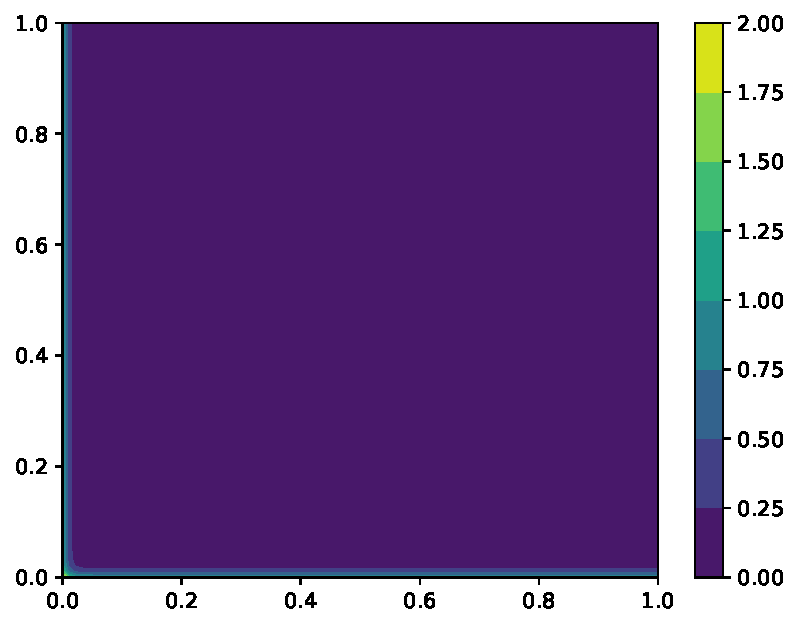
\includegraphics[width=0.32\linewidth]{ThesisFigs/bl2d_test.pdf}}
  \subfigure[\label{bl_2d_pred}SincKAN prediction]{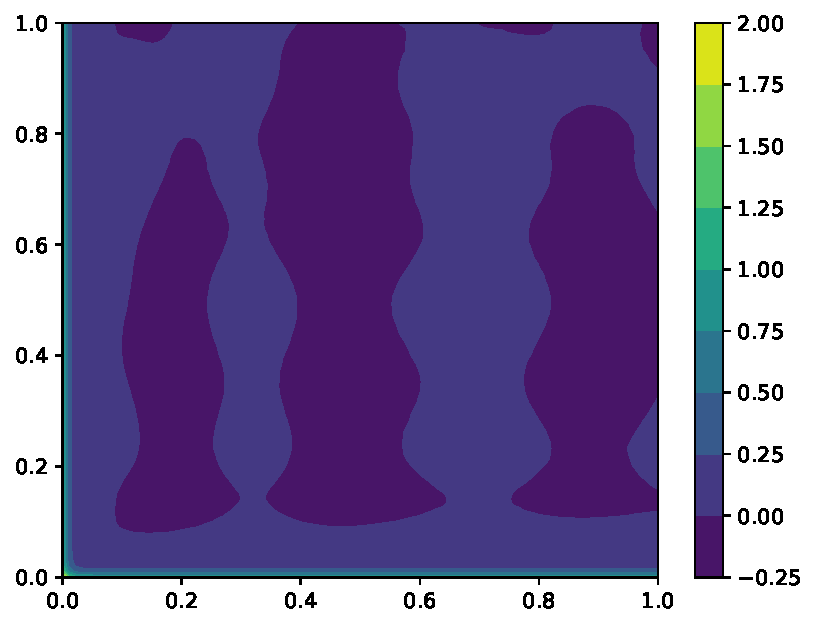
\includegraphics[width=0.32\linewidth]{ThesisFigs/bl2d_pred.pdf}}
  \subfigure[\label{bl_2d_error}Absolute error distribution]{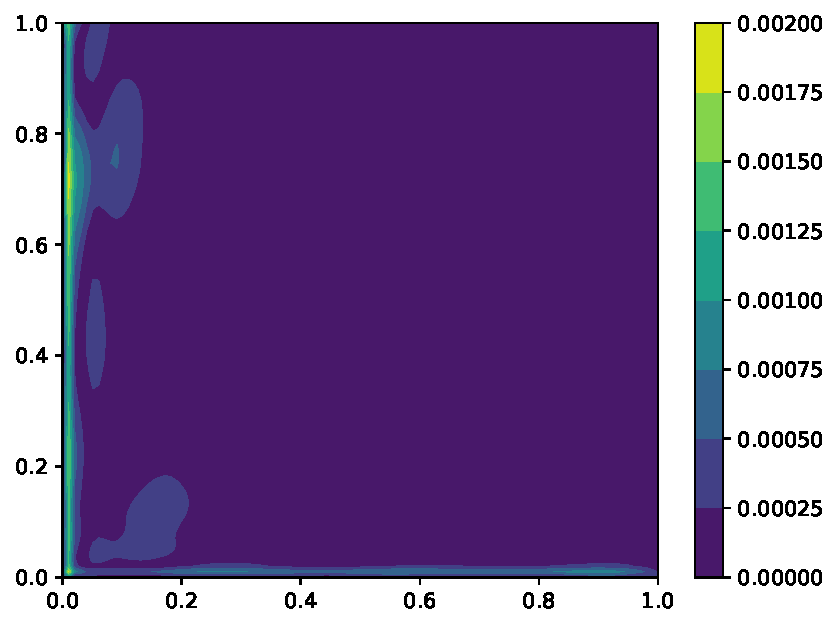
\includegraphics[width=0.32\linewidth]{ThesisFigs/bl2d_error.pdf}}
  \caption{Analysis of two-dimensional boundary layer problem: (a) exact solution of Equation~\ref{eq:bl2d}, (b) solution predicted by SincKAN, and (c) absolute error distribution, demonstrating that error concentrations primarily occur in the boundary layer region.}
  \label{fig:bl_2d}
\end{figure}

\subsubsection{Navier-Stokes Equations}
We examine the Taylor–Green vortex flow (components denoted as \textit{ns-tg-u} and \textit{ns-tg-v} in Table~\ref{table:pikan_pde}):
\begin{equation}
    \begin{gathered}
        \nabla \cdot \boldsymbol{u}=0, \quad t\in [0,T], \ \boldsymbol{x} \in \Omega,\\
        \partial_t \boldsymbol{u}+\boldsymbol{u} \cdot \nabla \boldsymbol{u}=-\nabla p+\nu\triangle \boldsymbol{u},\quad t\in [0,T], \ \boldsymbol{x} \in \Omega,
    \end{gathered}
\end{equation}
where $\boldsymbol{u}=(u,v)$. The system admits the exact solution:
\begin{equation}
    \begin{gathered}
        u = -\cos(x) \sin(y) \exp(-2\nu t), \\
        v = \sin(x) \cos(y) \exp(-2\nu t), \\
        p = -\left(\cos(2x) + \sin(2y)\right)\exp(-4\nu t)/4,
    \end{gathered}
\end{equation}
where $T=1$ and $\nu=1/400$. After non-dimensionalization, the spatial domain is $\boldsymbol{x} \in [0,1]^2$.

\section{Experimental Protocol}\label{Appendix: expeirment details}
All numerical experiments employ the Adam optimizer \citep{kingma2014adam} with exponential learning rate decay. The MLP and modified MLP architectures utilize hyperbolic tangent activation functions and Xavier initialization, following the methodology of \citet{raissi2019physics}.

\subsection{Function Approximation Protocol}
The hyperparameter configurations for the evaluated networks are presented in Table~\ref{table:cost for kans}. For one-dimensional problems, we implement the following protocol:

\begin{itemize}
    \item Training dataset generation: The input interval is uniformly discretized into 5000 points
    \item Training procedure: Each iteration randomly samples 3000 points from the training dataset
    \item Iteration count: Networks are trained for $10^5$ iterations
    \item Generalization assessment: Testing (fine) dataset comprises 10000 uniformly discretized points across the input interval
\end{itemize}

\subsection{PIKAN Implementation Protocol}
Network hyperparameters are specified in Table~\ref{table:cost for pikans}. The following protocols are implemented for different problem classes:

\begin{itemize}
    \item Time-independent one-dimensional problems:
    \begin{itemize}
        \item Training dataset: 1000 uniformly discretized points
        \item Sampling strategy: 500 random points per iteration
        \item Total iterations: $1.5 \times 10^6$
    \end{itemize}
    
    \item Time-dependent one-dimensional problems:
    \begin{itemize}
        \item Spatial discretization: 1000 points
        \item Temporal discretization: 11 points
        \item Sampling strategy: 5000 random points per iteration
        \item Total iterations: $1.5 \times 10^6$
    \end{itemize}
    
    \item Time-independent two-dimensional problems:
    \begin{itemize}
        \item Spatial discretization: 100 points per dimension
        \item Sampling strategy: 5000 random points per iteration
        \item Total iterations: $1.5 \times 10^6$
    \end{itemize}
    
    \item Time-dependent two-dimensional problems:
    \begin{itemize}
        \item Spatial discretization: 100 points per dimension
        \item Temporal discretization: 11 points
        \item Sampling strategy: 50000 random points per iteration
        \item Total iterations: $1.5 \times 10^6$
    \end{itemize}
    
    \item High-dimensional Poisson equation:
    \begin{itemize}
        \item Interior domain sampling: 2000 points per iteration
        \item Boundary domain sampling: 10000 points per iteration
        \item Test dataset composition: 8000 interior points and 2000 boundary points
        \item Total iterations: $5 \times 10^6$
    \end{itemize}
\end{itemize}

\subsection{Fractional PINN Implementation}\label{Appendix: fpinn}
Our implementation adopts the fPINNs framework \citep{pang2019fpinns}, utilizing the second-order Grünwald-Letnikov (GL) formula \citep{LISCHKE2020109009}:
\begin{equation}
(-\Delta)^{\alpha/2} u(x_j)=(1-\beta) \delta_{\Delta x, 1}^\alpha u(x_j)+\beta \delta_{\Delta x, 0}^\alpha u(x_j)+O((\Delta x)^2),
\end{equation}
where
\begin{equation}
\begin{aligned}
\delta_{\Delta x, p}^\alpha u(x_j) & :=(\Delta x)^{-\alpha} \sum_{k=0}^j(-1)^k\binom{\alpha}{k} u(x_j-(k-p) \Delta x)\\
& +(\Delta x)^{-\alpha} \sum_{k=0}^{N-j}(-1)^k\binom{\alpha}{k} u(x_j+(k-p) \Delta x).
\end{aligned}
\end{equation}

The computational domain $(0,1)$ is discretized with $\Delta x=1/N$, where $N=101$. We implement distinct learning rates: $10^{-2}$ for SincKAN and $10^{-3}$ for MLP. The networks are trained for $5\times10^5$ iterations, with SincKAN utilizing an architecture of $8\times 8 \times 1$. Performance metrics are presented in Figure~\ref{fig:frac_sol}.

\begin{figure}[ht]
  \centering
  \subfigure[$s=0.85$\label{sol_85}]{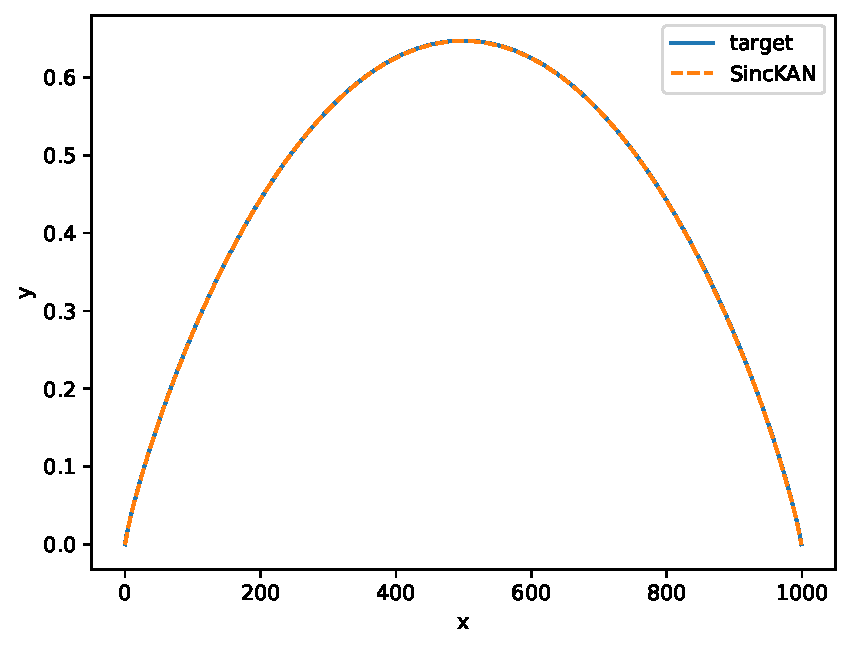
\includegraphics[width=0.32\linewidth]{ThesisFigs/frac_sol85.pdf}}
  \subfigure[$s=0.95$\label{sol_95}]{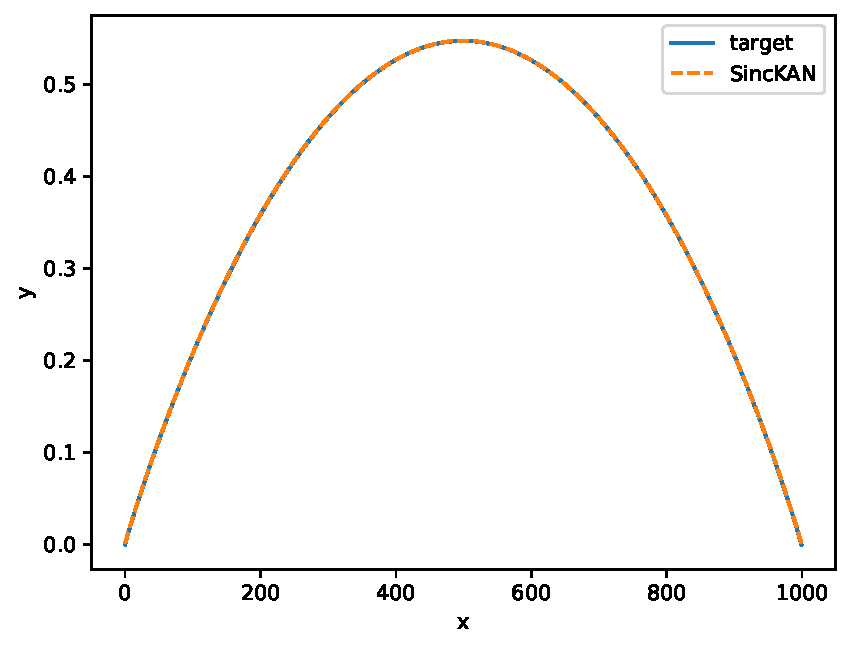
\includegraphics[width=0.32\linewidth]{ThesisFigs/frac_sol95.pdf}}
  \caption{Comparative analysis of target and SincKAN-predicted solutions for different fractional orders: (a) $s=0.85$ and (b) $s=0.95$.}
  \label{fig:frac_sol}
\end{figure}

\section{Analysis of SincKAN Interior Approximation}\label{Appendix: interior}
The internal approximation characteristics of SincKAN are demonstrated in Figure~\ref{fig:interior}.

\begin{figure}[ht]
   \centering
   \subfigure[\label{interior_approx}Equation~\ref{eq:bl2d} approximation analysis]{
\includegraphics[width=0.6\linewidth]{ThesisFigs/interior_approxi.pdf}}
   \subfigure[\label{interior_pde}PIKAN implementation analysis]{
\includegraphics[width=0.6\linewidth]{ThesisFigs/interior_pde.pdf}}
   \caption{Interior function analysis: (a) exhibits oscillatory behavior in interpolated $\phi$ due to high $M$ value implementation, while (b) demonstrates smoother $\phi$ characteristics resulting from low $M$ value implementation.}
   \label{fig:interior}
\end{figure}

\section{Generalization Analysis}\label{Appendix: fine grids}
As detailed in Section~\ref{Appendix: expeirment details}, we conduct additional evaluation on fine grid discretizations. Table~\ref{table: function fine grids} reveals certain limitations in SincKAN's generalization capabilities, suggesting areas for future research, although this limitation does not significantly impact the primary function approximation objectives.

\begin{table}[ht]
\caption{RMSE evaluated on fine grids}
\label{table: function fine grids}
\begin{center}
\begin{adjustbox}{width=\columnwidth, center}
\begin{tabular}{llllll}
\multicolumn{1}{c}{\bf Function name}  & \multicolumn{1}{c}{\bf MLP} & \multicolumn{1}{c}{\bf modified MLP} &\multicolumn{1}{c}{\bf KAN} & \multicolumn{1}{c}{\bf ChebyKAN} & \multicolumn{1}{c}{\bf SincKAN (ours)} 
\\ \hline 
\textit{sin-low} & $1.51 e\mbox{-}2 \pm 2.01 e\mbox{-}2$ & $7.29e\mbox{-}4 \pm 2.97 e\mbox{-}4$ & $1.27e\mbox{-}3 \pm 3.04e\mbox{-}4$ &
$1.76e\mbox{-}3 \pm 3.19e\mbox{-}4$ &
\textcolor{red}{$4.46 e\mbox{-}4 \pm 2.79 e\mbox{-}4$} \\ 
\textit{sin-high} & $7.07e\mbox{-}1 \pm 4.21e\mbox{-}8$ & $7.07 e\mbox{-}1 \pm 1.31 e\mbox{-}5$ & $7.06e\mbox{-}1 \pm 1.29e\mbox{-}3$ &
$5.70e\mbox{-}2 \pm 5.99 e\mbox{-}3$ &
\textcolor{red}{$4.15e\mbox{-}2 \pm 4.53e\mbox{-}3$} \\ 
\textit{bl} & $7.63e\mbox{-}4 \pm 1.13e\mbox{-}3$ & $5.72e\mbox{-}4 \pm 4.01e\mbox{-}4$ & $2.62e\mbox{-}4 \pm 7.89e\mbox{-}5$ &
$1.81e\mbox{-}3 \pm 6.98e\mbox{-}4$ &
\textcolor{red}{$2.28e\mbox{-}4 \pm 1.16e\mbox{-}4$} \\ 
\textit{double exponential} & $1.95e\mbox{-}3 \pm 8.17e\mbox{-}4$ & $7.76e\mbox{-}5 \pm 4.07e\mbox{-}5$ & $2.18e\mbox{-}4 \pm 1.51e\mbox{-}4$ &
$3.11e\mbox{-}3 \pm 2.16 e\mbox{-}3$ &
\textcolor{red}{$7.06e\mbox{-}5 \pm 1.09e\mbox{-}5$} \\ 
sqrt & $3.06e\mbox{-}3 \pm 9.34 e\mbox{-}4$ & \textcolor{red}{$4.46 e\mbox{-}5 \pm 5.51e\mbox{-}5$} & $4.79e\mbox{-}4 \pm 1.23e\mbox{-}4$ &
$3.69e\mbox{-}3 \pm 1.27 e\mbox{-}3$ &
$3.24e\mbox{-}4 \pm 1.31e\mbox{-}4$\\ 
\textit{multi-sqrt} & $2.06e\mbox{-}3 \pm 1.16e\mbox{-}3$ & $4.59e\mbox{-}4 \pm 4.86e\mbox{-}4$ & $3.61e\mbox{-}4 \pm 8.67 e\mbox{-}5$ &
$2.34e\mbox{-}3 \pm 1.17e\mbox{-}3$ &
\textcolor{red}{$2.14e\mbox{-}4 \pm 2.49 e\mbox{-}4$} \\ 
\textit{piece-wise} & $2.06e\mbox{-}2 \pm 5.57e\mbox{-}3$ & $3.75e\mbox{-}2 \pm 1.81e\mbox{-}2$ & $5.84e\mbox{-}2 \pm 1.03e\mbox{-}2$ &
\textcolor{red}{$7.28e\mbox{-}3 \pm 9.59 e\mbox{-}4$} &
$9.41e\mbox{-}3 \pm 2.14e\mbox{-}4$ \\ 
\textit{spectral-bias} & $2.48e\mbox{-}2 \pm 9.77 e\mbox{-}3$ & \textcolor{red}{$1.88e\mbox{-}2 \pm 9.55e\mbox{-}4$} & $4.79e\mbox{-}2 \pm 9.44 e\mbox{-}3$ &
$2.18e\mbox{-}2 \pm 2.97 e\mbox{-}4$ &
$2.21e\mbox{-}2 \pm 9.98 e\mbox{-}5$ \\ 
\end{tabular}
\end{adjustbox}
\end{center}
\end{table}

\section{Network Architecture Specifications}\label{Appendix: networks}
\subsection{Multilayer Perceptron}
The Multilayer Perceptron (MLP) architecture comprises fully connected neurons with nonlinear activation functions, expressed mathematically as:
\begin{equation}
\operatorname{MLP}(x)=\left(W^{L-1} \circ \sigma \circ W^{L-2} \circ \sigma \circ \cdots \circ W^1 \circ \sigma \circ W^0\right) \vx,
\end{equation}
where $W^i(x)=W_ix+b_i$, with $W_i \in \mathbb{R}^{m_i \times n_i}$ representing learnable matrices, $b_i \in \mathbb{R}^{m_i}$ denoting learnable bias terms, $\sigma$ representing the chosen nonlinear activation function, and $L$ indicating network depth.

\subsection{Modified MLP}
The Modified MLP architecture, inspired by transformer networks, incorporates two additional features with skip connections:
\begin{equation}
\begin{gathered}
    U=\sigma(W^{L+1}\vx), \quad V=\sigma(W^{L+2}\vx), \quad H^1=\sigma(W^{0}\vx), \\
    H^{i+1} = (1-\sigma(W^{i}H^{i}))*U+\sigma(W^{i}H^{i})*V, \quad i=1,\dots,L, \\
    \operatorname{Modified MLP}(\vx) = W^{L+3}H^{L+1},
\end{gathered}
\end{equation}
where $*$ denotes element-wise multiplication.

\subsection{Kolmogorov-Arnold Network}\label{Appendix: networks_kan}
\subsubsection{Theoretical Foundation}
The Kolmogorov-Arnold representation theorem establishes that any continuous multivariate function on a bounded domain can be represented through finite composition of univariate continuous functions and addition. Specifically, for a continuous function $f:[0,1]^n\rightarrow \mathbb{R}$, there exist continuous univariate functions $\phi_{q,p}$ and $\Phi_{q}$ such that:
\begin{equation}
    f(\mathbf{x})=f(x_1, \dots, x_n)=\sum_{q=1}^{2n+1} \Phi_q\left(\sum_{p=1}^n \phi_{q,p}(x_p)\right).
\end{equation}

\subsubsection{Architectural Implementation}
The Kolmogorov-Arnold Network (KAN) extends traditional neural architectures by implementing learnable activation functions. Let $\mathbf{\Phi}=\{\phi_{p,q}\}$ represent a matrix of univariate functions where $p= 1, 2, \dots n_{in}, q= 1, 2, \dots n_{out}$, and $\theta$ denote trainable parameters. The KAN is defined as:
\begin{equation}
    \operatorname{KAN} (\vx) = \left(\mathbf{\Phi}_{L-1} \circ \mathbf{\Phi}_{L-2} \circ \cdots \circ \mathbf{\Phi}_1 \circ \mathbf{\Phi}_0\right) \vx, \quad \vx\in \mathbb{R}^d,
\end{equation}
where:
\begin{equation}\label{eq: def phi}
\mathbf{\Phi}_{l}(\vx^{(l)})= \left\{\sum_{i=1}^{n^{(l)}_{in}} \phi_{j,i}(x_{i}^{(l)})\right\}_{j=1}^{n^{(l)}_{out}}, \quad \forall l = 0,1,\dots,L-1,
\end{equation}
with $\vx^{l} \in \mathbb{R}^{n_{in}^{(l)}}$ and $\mathbf{\Phi}_{l}(\vx^{(l)}) \in \mathbb{R}^{n_{out}^{(l)}}$. For a KAN of size $[n_0,n_1,\dots,n_L]$, we have $n^{(l)}_{in}=n_l$ and $n^{(l)}_{out}=n_{l+1}$.

Each activation function $\phi$ is approximated through a combination of basis functions and spline interpolation:
\begin{equation}
    \phi(x)=w_b \mathrm{silu}(x)+w_s \left(\sum_i^N c_i B_i(x)\right),
\end{equation}
where $c_i$, $w_s$, and $w_b$ are learnable parameters, $B_i$ represents the $k$-th order B-splines, $N=G+k-1$, and $G$ denotes the grid size.

\subsection{ChebyKAN Architecture}
The ChebyKAN architecture implements Chebyshev polynomials for the construction of learnable activation functions within the KAN framework. The modified ChebyKAN variant incorporates hyperbolic tangent activation functions between successive layers, yielding the following architectural formulation:
\begin{equation}
    \operatorname{ChebyKAN} (\vx) = \left(\mathbf{\Phi}_{L-1} \circ \tanh \circ \mathbf{\Phi}_{L-2}\circ \cdots \circ \mathbf{\Phi}_1 \circ \tanh \circ \mathbf{\Phi}_0\circ \tanh\right) \vx, \quad \vx\in \mathbb{R}^d,
\end{equation}
where $\mathbf{\Phi}$ maintains the definition from Equation~\ref{eq: def phi} with univariate functions:
\begin{equation}
    \phi = \sum_i c_i T_i(x),
\end{equation}
where $T_i$ represents the $i$-th Chebyshev polynomial.

\section{Computational Cost Analysis}\label{Appendix: cost}
\subsection{Training Complexity}
The SincKAN architecture, as defined in Equation~\ref{eq: Sinc activation function}, incorporates an additional summation over multiple step sizes $h$, resulting in trainable coefficients $c$ that are $M$ times larger than those in KAN and ChebyKAN implementations. However, total training time depends on multiple factors beyond parameter count. Tables~\ref{table:cost for kans} and \ref{table:cost for pikans} present comprehensive computational costs for approximation and PDE tasks, respectively.

In these tables, we employ the following notation conventions:
- MLP and modified MLP architectures: 'depth$\times$width'
- KAN and ChebyKAN architectures: 'width$\times$degree'
- SincKAN architecture: 'width$\times$degree$\times M

Network training was conducted in two distinct computational environments:
\begin{itemize}
    \item \dag: Single NVIDIA A100-SXM4-80GB GPU, CUDA version 12.4
    \item \ddag: Single NVIDIA A40-48GB GPU, CUDA version 12.4
\end{itemize}

\begin{table}[ht]
\caption{Computational Cost Analysis for Approximation Tasks\dag}
\label{table:cost for kans}
\begin{center}
\begin{tabular}{lllll}
\multicolumn{1}{c}{\textbf{Network}} & \multicolumn{1}{c}{\textbf{Architecture}} & \multicolumn{1}{c}{\textbf{Training Rate (iter/sec)}} & \multicolumn{1}{c}{\textbf{Reference Time (ms)}} & \multicolumn{1}{c}{\textbf{Parameters}} \\ \hline
MLP & $10\times 100$ & $9.89\times 10^2$ & $1.62\times 10^1$ & $81,101$ \\
Modified MLP & $10\times 100$ & $9.13\times 10^2$ & $2.92\times 10^1$ & $81,501$ \\
KAN & $8\times 8$ & $1.15\times 10^3$ & $1.01\times 10^2$ & $160$ \\
ChebyKAN & $40\times 40$ & $1.29\times 10^3$ & $3.11\times 10^1$ & $3,280$ \\
SincKAN & $8\times 100 \times 6$ & $1.29\times 10^3$ & $2.06\times 10^1$ & $9,696$ \\
\end{tabular}
\end{center}
\end{table}

\begin{table}[ht]
\caption{Computational cost for train PIKANs}
\label{table:cost for pikans}
\begin{center}
\begin{tabular}{lllll}
\multicolumn{1}{c}{\bf Function name}  & \multicolumn{1}{c}{\bf Network}& \multicolumn{1}{c}{\bf Size}  & \multicolumn{1}{c}{\bf Training rate (iter/sec)} & \multicolumn{1}{c}{\bf Parameters} \\ 
\hline 
\multirow{5}{*}{boundary layer$^\ddag$ } & MLP &$10\times 100$ & $6.47\times 10^{2}$ & 81101 \\
                      & modified MLP & $10\times 100$ &$3.55\times 10^{2}$ & 81501\\ 
                      & KAN & $8\times 8$  &$1.33\times 10^{3}$ & 160\\ 
                      & ChebyKAN & $40\times 40$ & $1.89\times 10^{3}$  & 3280\\ 
                      & SincKAN & $8\times 8 \times 1$ & $1.27\times 10^{3}$  & 194 \\ 
\\
\multirow{5}{*}{\textit{perturbed}$^\ddag$ } & MLP & $10\times 100$ & $6.85\times 10^{2}$ & 81101 \\ 
                      & modified MLP &$10\times 100$ & $3.59\times 10^{2}$ & 81501\\ 
                      & KAN & $8\times 8$ & $1.27\times 10^{3}$ & 160\\ 
                      & ChebyKAN & $40\times 40$ & $1.07\times 10^{3}$ & 3280 \\ 
                      & SincKAN & $8\times 8 \times 1$ & $1.25\times 10^{3}$ &194 \\ 
\\
\multirow{5}{*}{\textit{nonlinear}$^\ddag$ } & MLP & $10\times 100$ & $4.62\times 10^{2}$ & 81101\\ 
                      & modified MLP & $10\times 100$ & $3.07\times 10^{2}$ & 81501\\ 
                      & KAN & $8\times 8$ & $1.56\times 10^{3}$ & 160\\ 
                      & ChebyKAN & $40\times 40$ & $1.53\times 10^{3}$ & 3280 \\ 
                      & SincKAN & $8\times 4 \times 1$ & $1.54\times 10^{3}$ & 130 \\ 
\\
\multirow{5}{*}{\textit{bl-2d}$^\ddag$ } & MLP & $10\times 100$ & $2.39\times 10^{2}$ & 81201\\ 
                      & modified MLP & $10\times 100$ & $1.96\times 10^{2}$ & 81801\\ 
                      & KAN & $8\times 8$ & $3.46\times 10^{2}$ & 240\\ 
                      & ChebyKAN & $40\times 40$ & $4.95\times 10^{2}$ & 4920 \\ 
                      & SincKAN & $8\times 20 \times 1$ & $2.97\times 10^{2}$ & 570 \\ 
\\
\multirow{5}{*}{\textit{ns-tg}$^\dag$ } & MLP & $10\times 100$ & $1.71\times 10^{2}$ & 81503\\ 
                      & modified MLP & $10\times 100$ & $1.51\times 10^{2}$ & 82303\\ 
                      & KAN & $8\times 8$ & $2.55\times 10^{2}$ & 480\\ 
                      & ChebyKAN & $40\times 40$ & $3.83\times 10^{3}$ & 9840 \\ 
                      & SincKAN & $8\times 8 \times 1$ & $2.77\times 10^{2}$ & 550 \\ 
\end{tabular}
\end{center}
\end{table}

\subsection{Reference Time Analysis}
The computational cost of reference operations exhibits independence from the specific task formulation (i.e., the loss function). Results evaluated on models trained for approximation tasks are presented in Table~\ref{table:cost for kans}. Despite SincKAN's larger parameter count compared to KAN and ChebyKAN, it demonstrates superior reference operation efficiency. This performance advantage is attributable to the compilation of training procedures using JAX~\cite{jax2018github}, which optimizes computational operations.

\section{Degree-Data Size Relationship Analysis}\label{Appendix: scaling law}
In traditional Sinc numerical methods, the number of sampled points equals the degree ($N_{degree}=N_{points}$), as each degree requires a corresponding function value $f(jh)$ at point $jh$. However, this equivalence proves impractical and unnecessary in the SincKAN framework, where multi-layer representation provides exponentially increasing capacity with depth \citep{yarotsky2017error}. To investigate the relationship between degree and data size, we conducted a comprehensive empirical analysis of SincKAN performance under varying $N_{degree}$ and $N_{points}$ configurations.

The experimental protocol employed the \textit{spectral-bias} function with the following parameter space:
\begin{itemize}
    \item Degrees: $N \in \{8,16,32,64,100,300\}$
    \item Data points: $N_{points} \in \{100,500,1000,5000,10000\}$
    \item Batch size adaptation: $N_{batch}=N_{points}/4$
\end{itemize}

Additional parameters were fixed at:
\begin{itemize}
    \item Inverse decay sequence: $\{h_i\}_{i=1}^M$ with $M=6$
    \item Base step size: $h_0=7.0$
\end{itemize}

Results are presented in Table~\ref{table: degree_points} and visualized in Figure~\ref{fig:degree_points}. Of particular note, Figure~\ref{degree_100} demonstrates that our neural scaling follows $\mathrm{RMSE} \propto G^{-4}$, surpassing the best scaling law $\mathrm{RMSE} \propto G^{-3}$ reported in KAN~\citep{liu2024kan}.
\begin{table}[ht]
\caption{RMSE for different degree and $N_{points}$}
\label{table: degree_points}
\begin{center}
\begin{adjustbox}{width=\columnwidth, center}
\begin{tabular}{clllll}
degree $\setminus$ $N_{points}$& \multicolumn{1}{c}{100} &\multicolumn{1}{c}{500} & \multicolumn{1}{c}{1,000} & \multicolumn{1}{c}{5,000} & \multicolumn{1}{c}{10,000}
\\ \hline
8 &$2.60e\mbox{-}1 \pm 2.76e\mbox{-}5$     & $1.16e\mbox{-}1 \pm 6.34e\mbox{-}6$   & $8.23e\mbox{-}2 \pm 4.54e\mbox{-}6$ & $6.70e\mbox{-}2 \pm 3.91e\mbox{-}3$ & $6.81e\mbox{-}2 \pm 4.51e\mbox{-}3$ \\
16                         & $1.01e\mbox{-}2 \pm 1.47e\mbox{-}2$  & $1.30e\mbox{-}3 \pm 9.42e\mbox{-}4$   & $1.04e\mbox{-}3 \pm 3.74e\mbox{-}4$ & $1.62e\mbox{-}3 \pm 2.48e\mbox{-}4$ & $9.57e\mbox{-}4 \pm 4.35e\mbox{-}4$ \\
32                         & \textcolor{red}{$3.63e\mbox{-}5 \pm 5.79e\mbox{-}5$}   & $2.69e\mbox{-}4 \pm 2.27e\mbox{-}4$   & $4.72e\mbox{-}4 \pm 2.75e\mbox{-}4$ & $2.15e\mbox{-}3 \pm 1.57e\mbox{-}3$ & $3.08e\mbox{-}3 \pm 7.14e\mbox{-}4$ \\
  64                       & $1.29e\mbox{-}3 \pm 2.21e\mbox{-}3$  & $5.60e\mbox{-}4 \pm 6.42e\mbox{-}4$   & $2.74e\mbox{-}3 \pm 4.01e\mbox{-}3$ & $1.83e\mbox{-}3 \pm 8.49e\mbox{-}4$ & $2.13e\mbox{-}3 \pm 9.05e\mbox{-}4$ \\
100 &$7.66e\mbox{-}5 \pm 1.16e\mbox{-}4$    & $3.79e\mbox{-}4 \pm 6.27e\mbox{-}4$  & $4.24e\mbox{-}4 \pm 7.42e\mbox{-}5$ & $2.19e\mbox{-}3 \pm 1.62e\mbox{-}3$ & $2.64e\mbox{-}3 \pm 1.76e\mbox{-}3$  \\ 
 300                        & $3.73e\mbox{-}4 \pm 5.62e\mbox{-}4$  &  $7.30e\mbox{-}5 \pm 4.25e\mbox{-}5$ & $7.54e\mbox{-}4 \pm 8.73e\mbox{-}4$ & $2.21e\mbox{-}3 \pm 1.04e\mbox{-}3$ & $2.18e\mbox{-}3 \pm 1.12e\mbox{-}3$  \\ 
\end{tabular}
\end{adjustbox}
\end{center}
\end{table}

\begin{figure}[ht]
  \centering
  \subfigure[\label{degree_100}$N_{points}=100$]{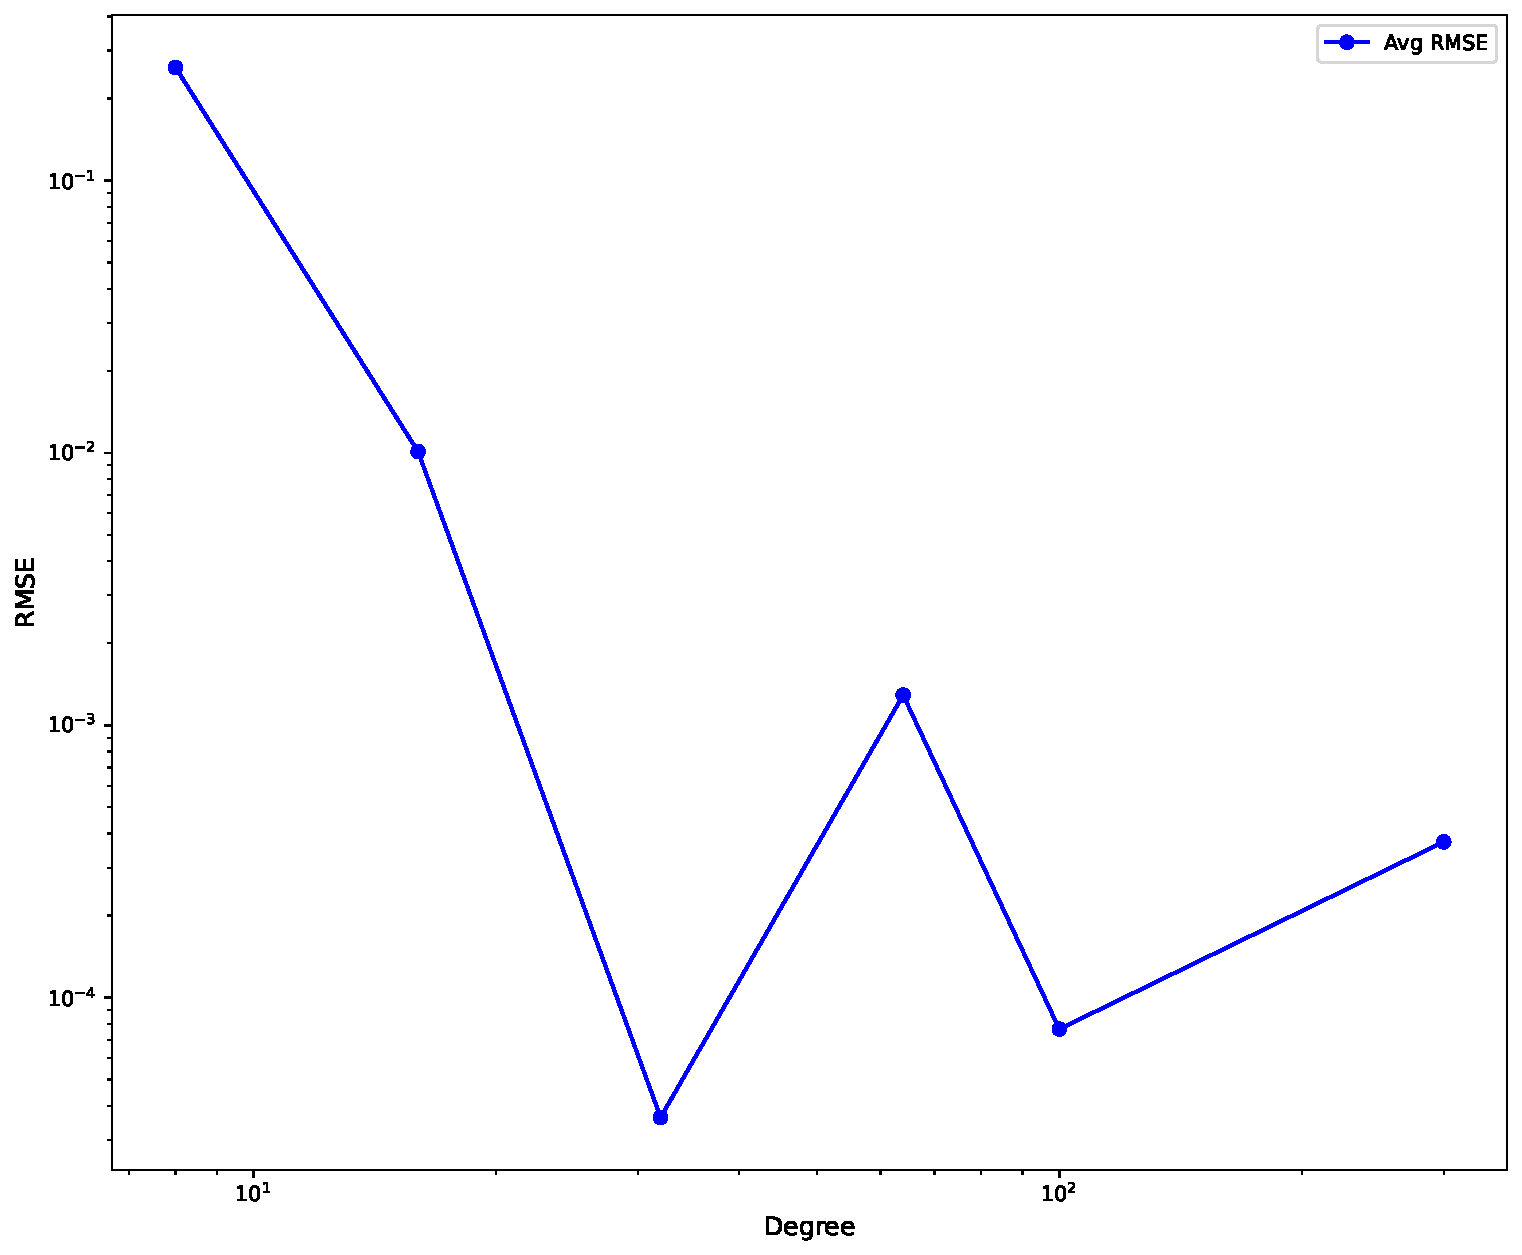
\includegraphics[width=0.3\linewidth]{ThesisFigs/degree_npoint_100.pdf}}
  \subfigure[\label{degree_500}$N_{points}=500$]{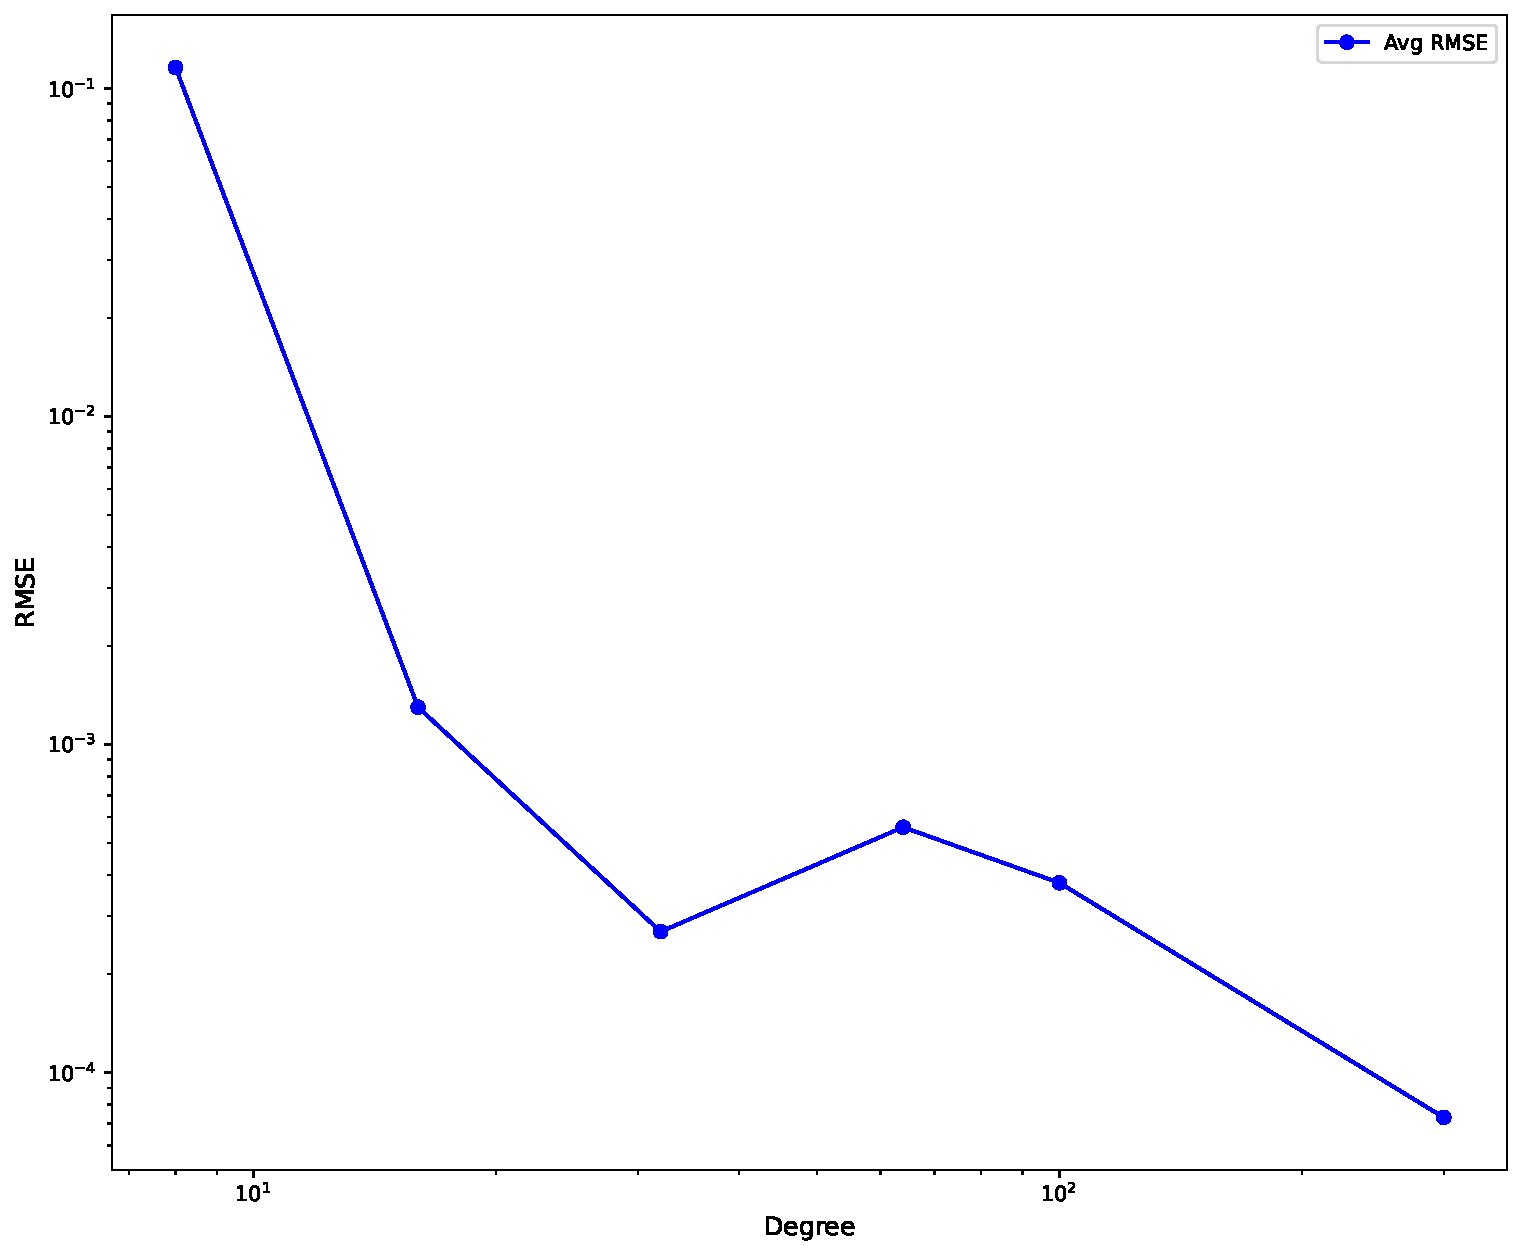
\includegraphics[width=0.3\linewidth]{ThesisFigs/degree_npoint_500.pdf}}
  \subfigure[\label{degree_1000}$N_{points}=1000$]{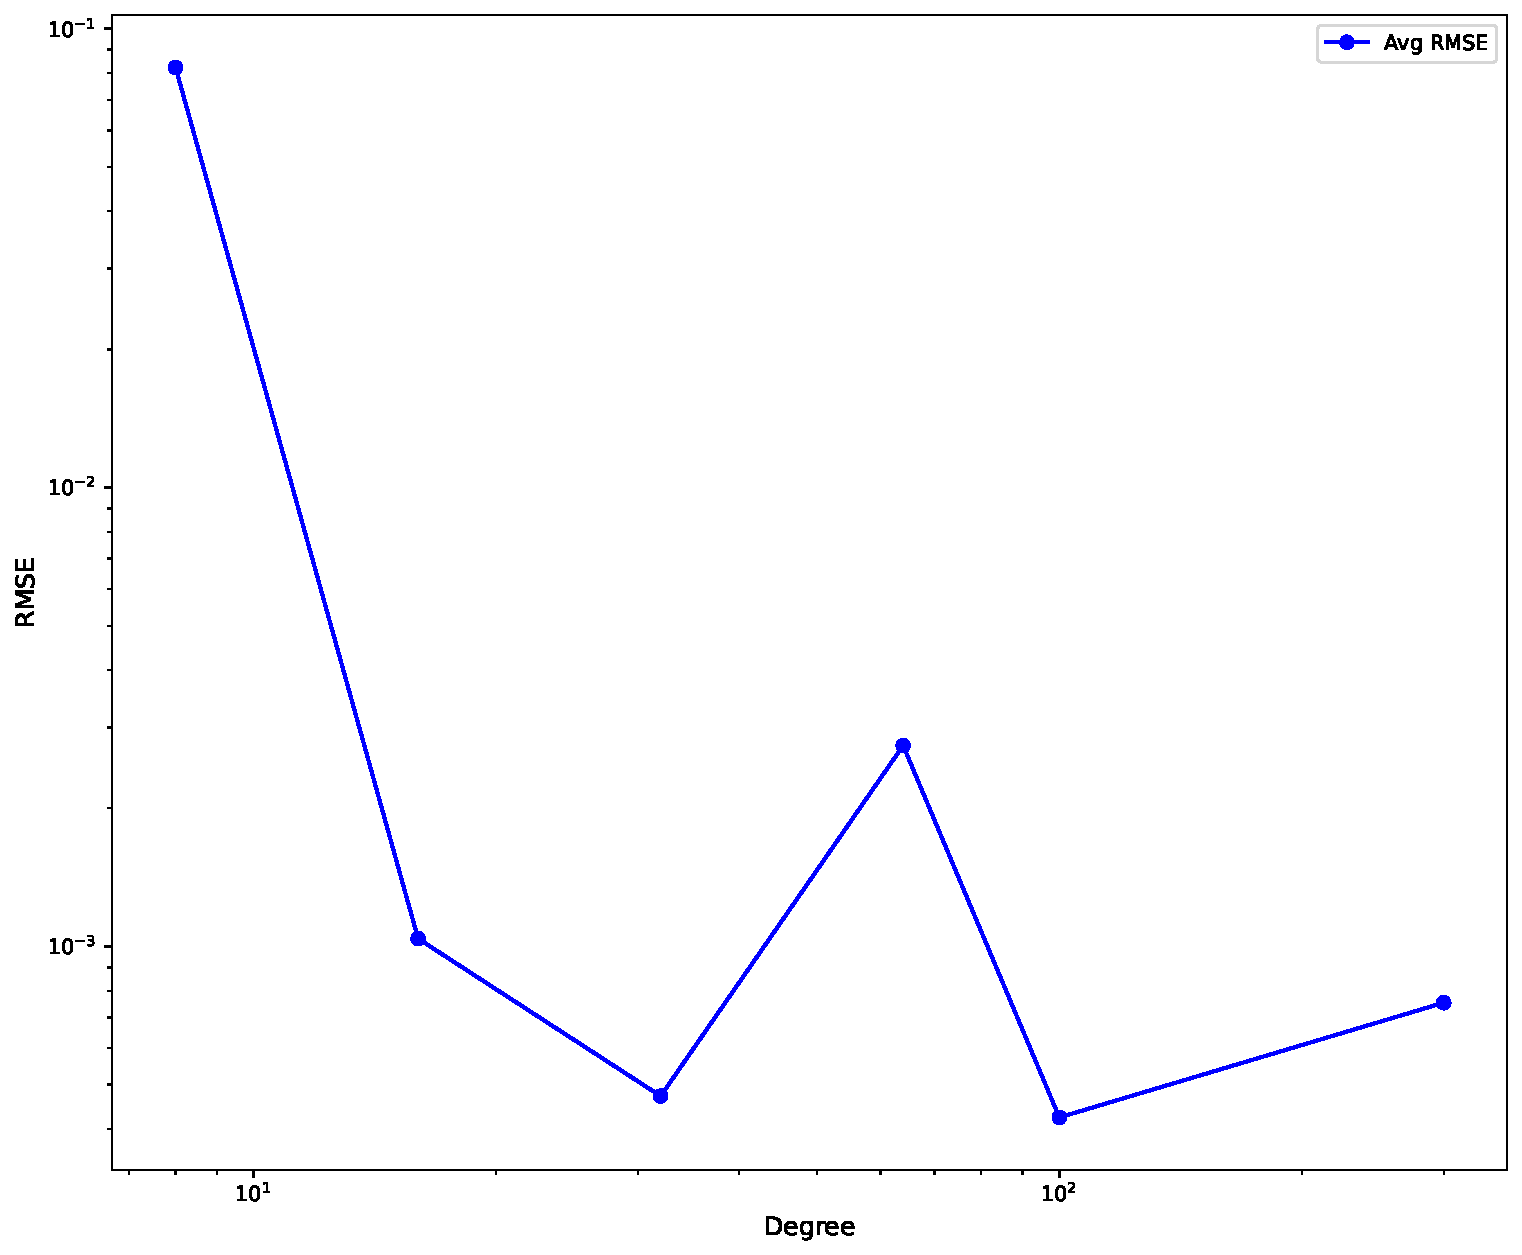
\includegraphics[width=0.3\linewidth]{ThesisFigs/degree_npoint_1000.pdf}}
  \subfigure[\label{degree_5000}$N_{points}=5000$]{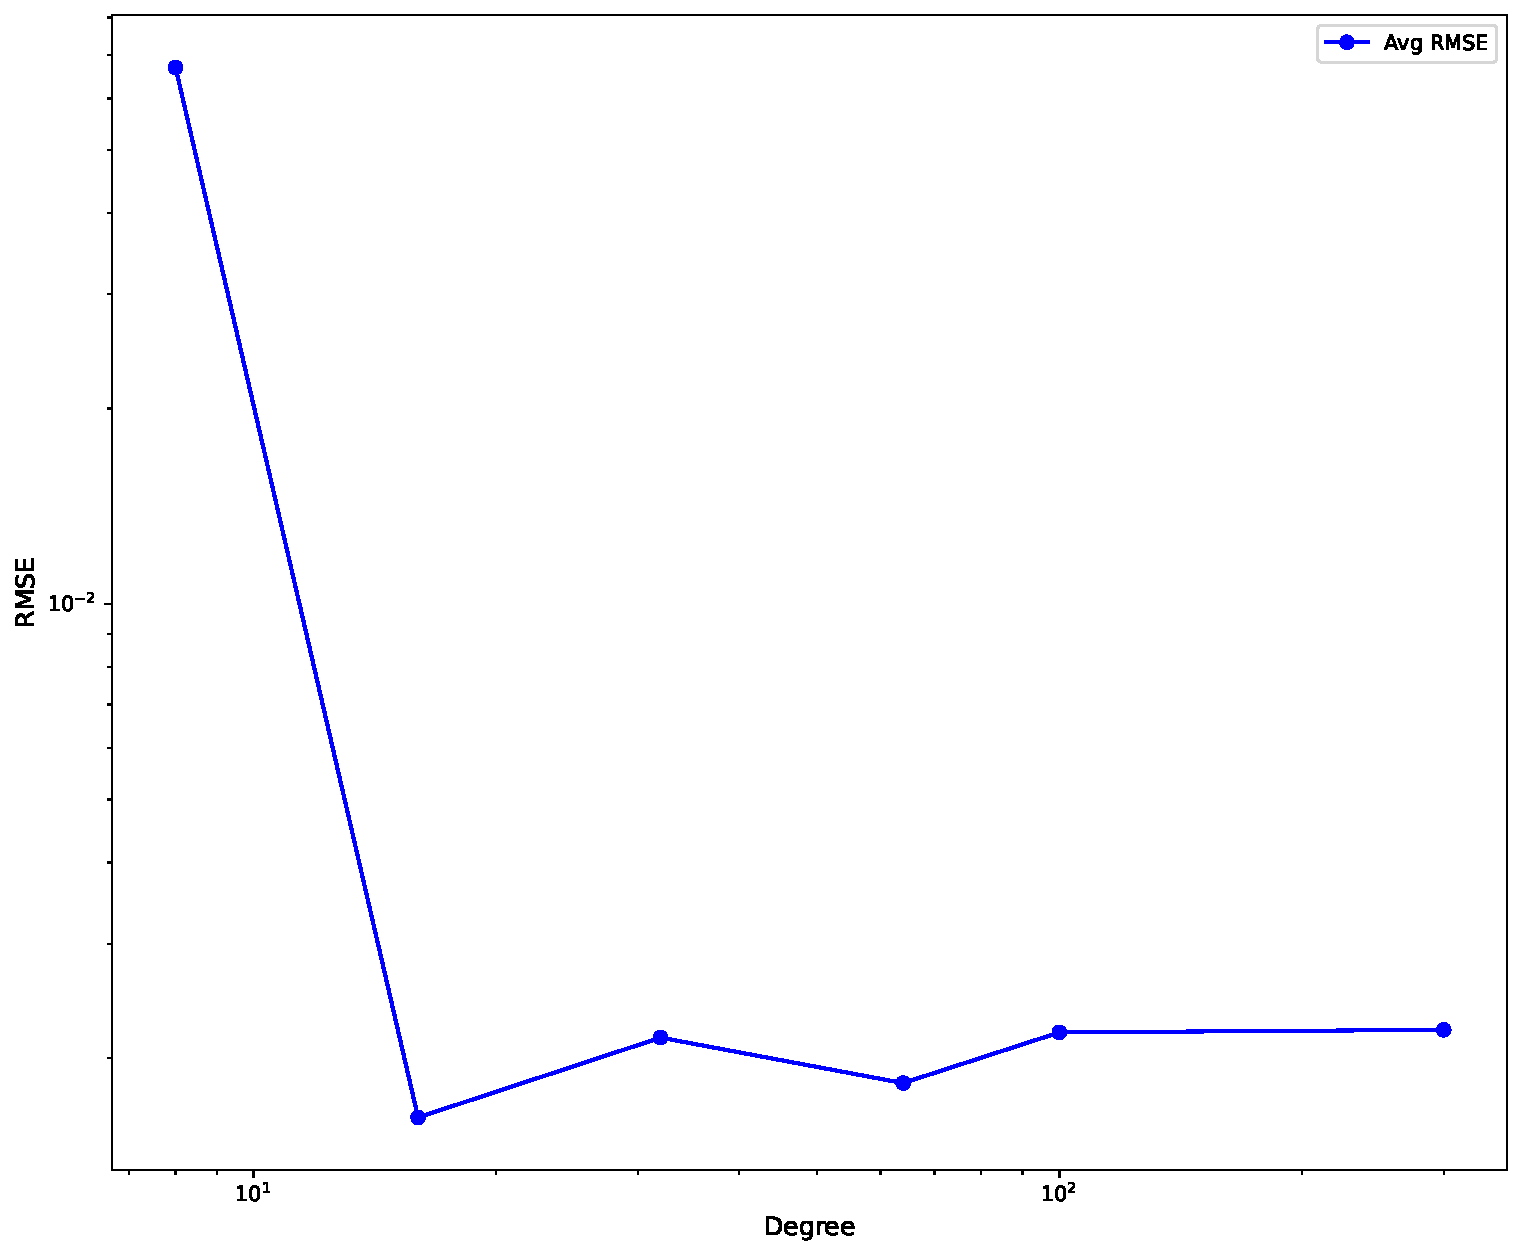
\includegraphics[width=0.3\linewidth]{ThesisFigs/degree_npoint_5000.pdf}}
  \subfigure[\label{degree_10000}$N_{points}=10000$]{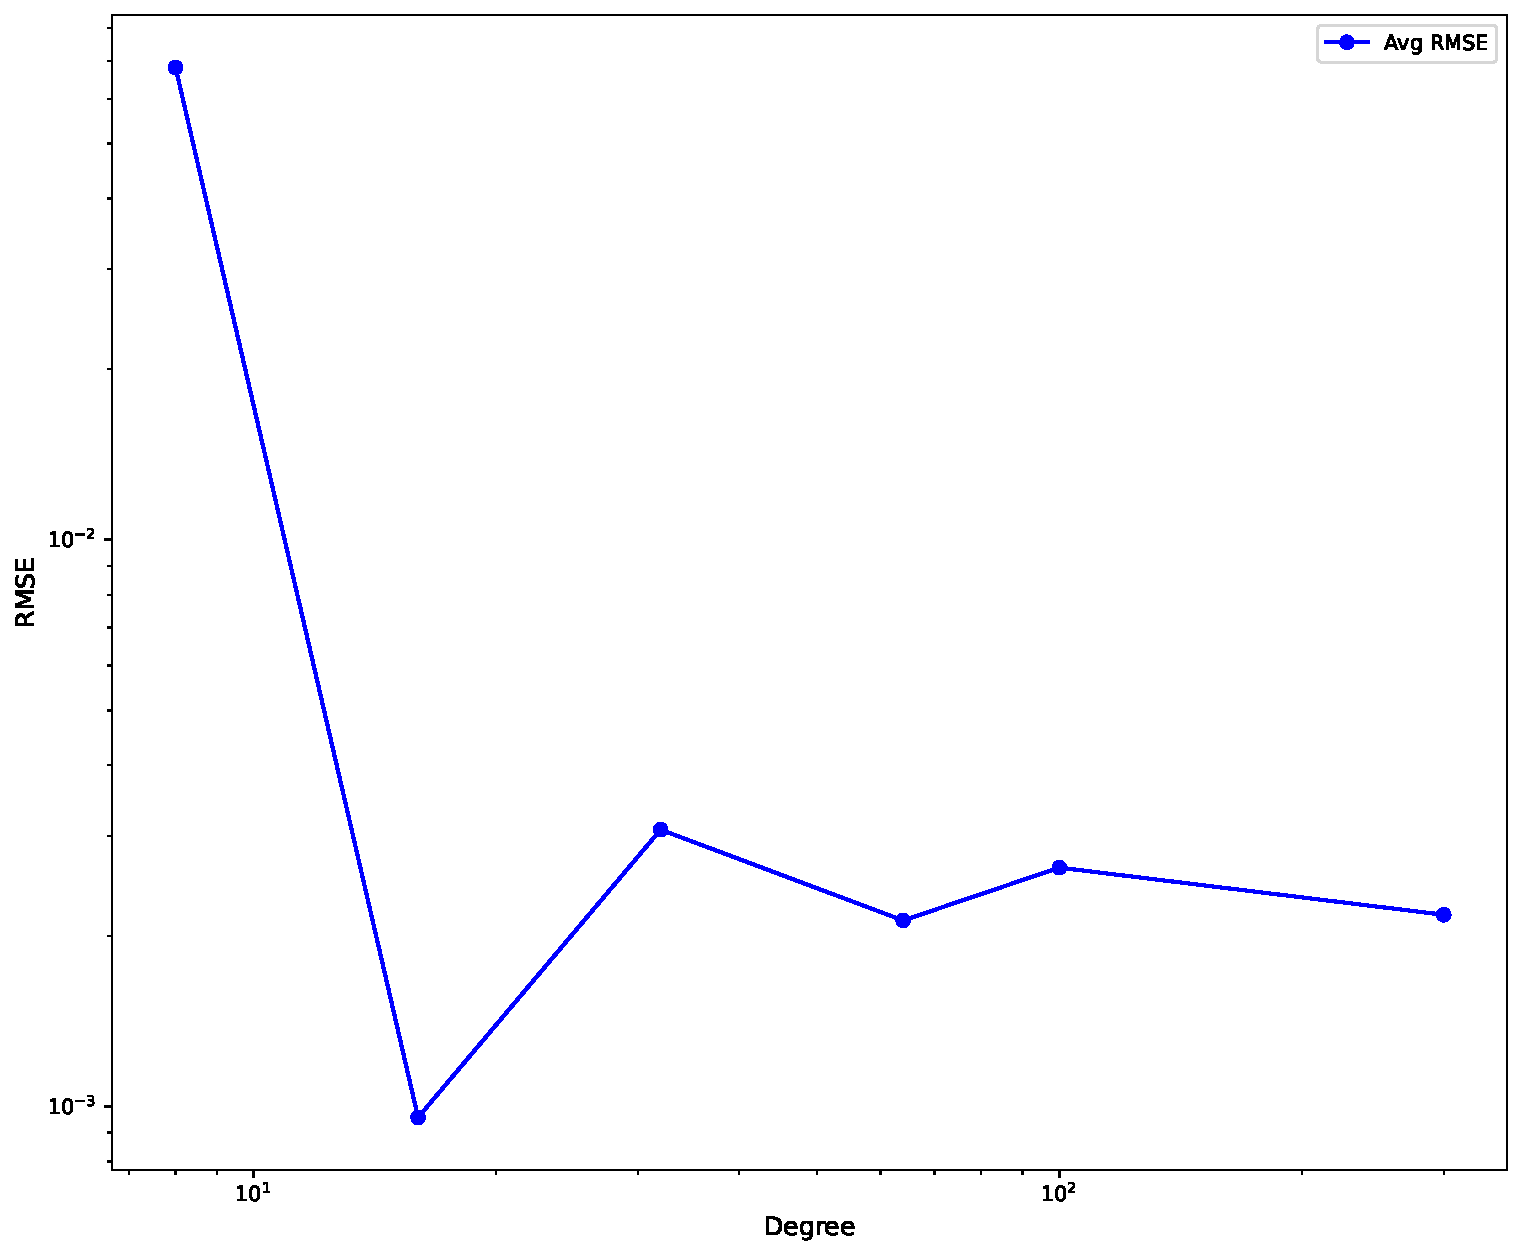
\includegraphics[width=0.3\linewidth]{ThesisFigs/degree_npoint_10000.pdf}}
  \caption{Performance analysis across varying $N_{points}$ configurations with increasing degree specifications.}
  \label{fig:degree_points}
\end{figure}

\section{Basis Update Strategy}\label{Appendix: update}
The interpolation methodology for each $\phi$ component represents a critical element of KAN architectures. However, the optimal degree for interpolation methods typically requires empirical determination. Table~\ref{table: degree_points} demonstrates that increased degree does not necessarily correlate with improved accuracy, potentially due to over-parameterization effects. To address this limitation, we propose Algorithm~\ref{algorithm: grids} for grid extension, enabling SincKAN to progress from small to large degrees adaptively.

\begin{algorithm}[ht]
   \caption{Grid Extension Protocol}
   \label{algorithm: grids}
   \begin{algorithmic}[1] 
       \Require $M > N > 0, \{c_i\}_{i=-N}^{N}$
       \Ensure $\{c^\prime_i\}_{i=-M}^{M}$
       \For{$i = -M$ \textbf{to} $M$}
           \If{$i \in [-N, N]$}
               \State $c_i^\prime \gets c_i$
           \Else
               \State $c_i^\prime \gets 0$
           \EndIf
       \EndFor
   \end{algorithmic}
\end{algorithm}
This methodology was evaluated using identical hyperparameters as described in \cref{Appendix: scaling law}, specifically focusing on \textit{spectral-basis} and \textit{bl} functions. In the initial experiment, a constant degree of $N_{degree}=100$ was established. For the variable degree implementation, the initialization began at $N_{degree}=8$, with subsequent updates following the sequence $\left[8, 8, 8, 8, 8, 8, 8, 8, 8, 8, 4, 4, 4\right]$ over 13 iterations until reaching $N_{degree}=100$. The constant degree model underwent training for $1.4\times 10^6$ iterations. In the variable degree configuration, each degree was trained for $10^5$ iterations, maintaining a cumulative training duration of $1.4\times10^6$ iterations, with the resultant grid updates illustrated in \cref{fig:update}. Upon observation of potential overfitting at $N_{degree}=100$, a second experiment was conducted with a reduced constant degree of $N_{degree}=96$. The variable degree implementation in this case commenced at $N_{degree}=8$, with progressive updates of $\left[8, 8, 8, 8, 8, 8, 8, 8, 8, 8, 4, 4\right]$ over 13 iterations until achieving $N_{degree}=96$. The constant degree model underwent training for $1.3\times 10^6$ iterations, while the variable degree configuration maintained $10^5$ iterations per degree, resulting in an equivalent total of $1.3\times10^6$ iterations. The corresponding grid updates are presented in \cref{fig:update_96}.
It is noteworthy that the computational efficiency of the variable degree approach marginally exceeds that of the constant degree method, owing to the optimization of basis changes. The comparative computational costs are detailed in \cref{table:cost for update}.
\begin{figure}[ht]%[H]%
\centering %%$u_t = \epsilon{\partial^6 u\over \partial x^6}$ %%$u_t = \epsilon{\partial^{10} u\over \partial x^{10}}$
\subfigure[\textit{bl}\label{update_bl_no}]{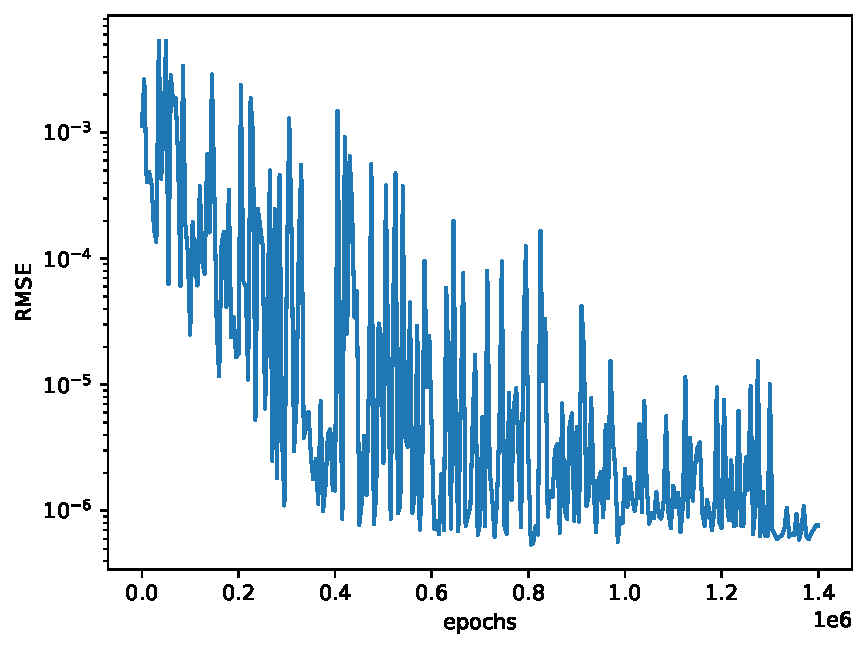
\includegraphics[width=0.42\linewidth]{ThesisFigs/bl_RMSE_001.pdf}}
\subfigure[\textit{bl}\label{update_bl_noinit}]{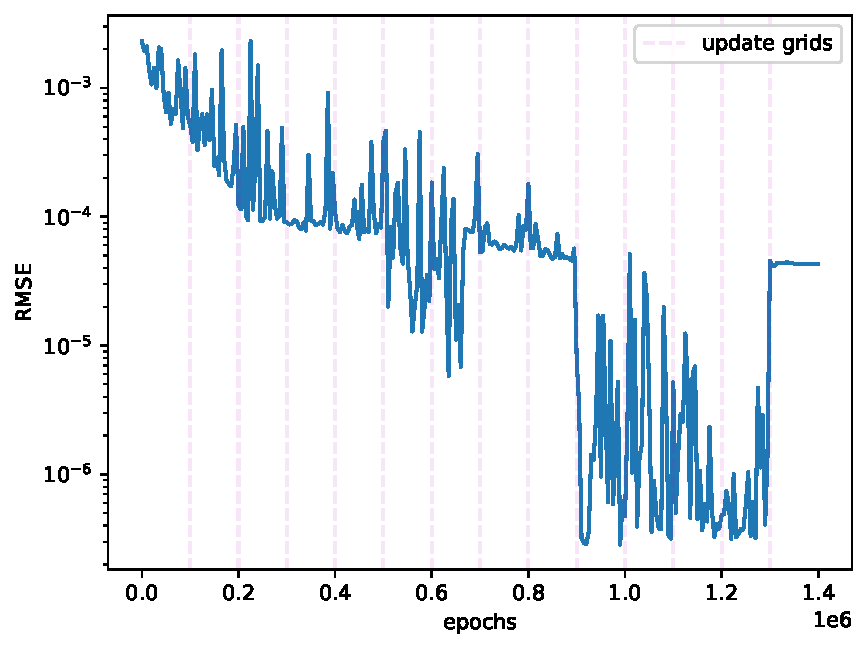
\includegraphics[width=0.42\linewidth]{ThesisFigs/bl_RMSE_010.pdf}}
\subfigure[\textit{spectral-basis}\label{update_sb_no}]{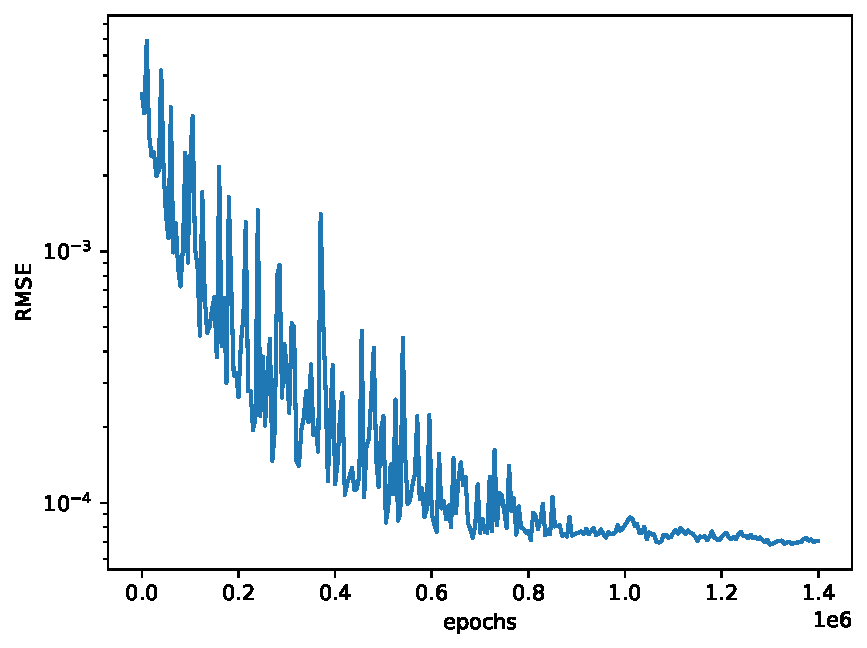
\includegraphics[width=0.42\linewidth]{ThesisFigs/sb_RMSE_001.pdf}}
\subfigure[\textit{spectral-basis}\label{update_sb_noinit}]{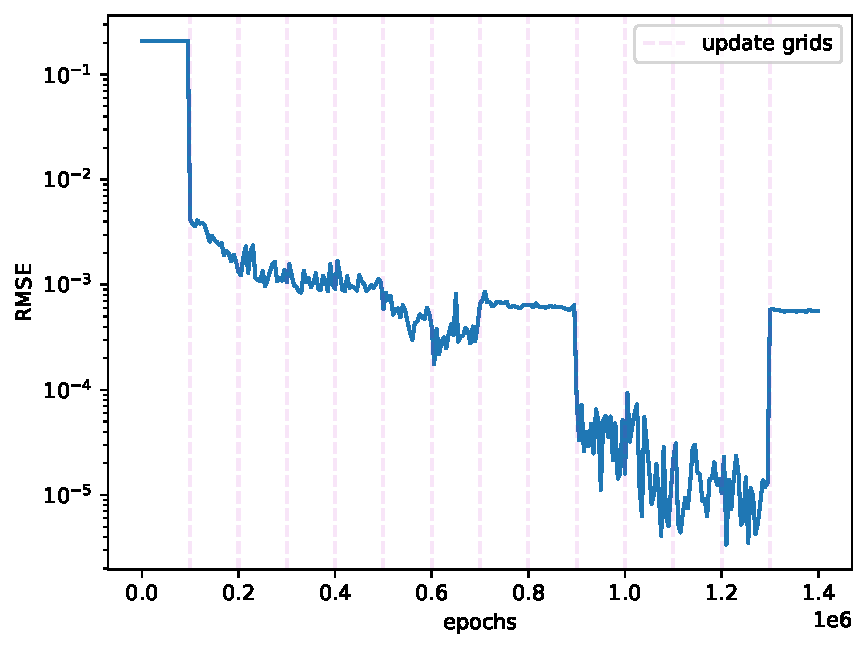
\includegraphics[width=0.42\linewidth]{ThesisFigs/sb_RMSE_010.pdf}}
\caption{For \textit{bl} and \textit{spectral-basis}, \cref{update_bl_no} and \cref{update_sb_no} correspondingly shows the RMSE for the constant degree $N_{degree}=100$; \cref{update_bl_noinit} and \cref{update_sb_noinit} correspondingly shows the RMSE for the variable degree}
\label{fig:update}
\end{figure}
\begin{figure}[ht]%[H]%
\centering %%$u_t = \epsilon{\partial^6 u\over \partial x^6}$ %%$u_t = \epsilon{\partial^{10} u\over \partial x^{10}}$
\subfigure[\textit{bl}\label{update_bl_no96}]{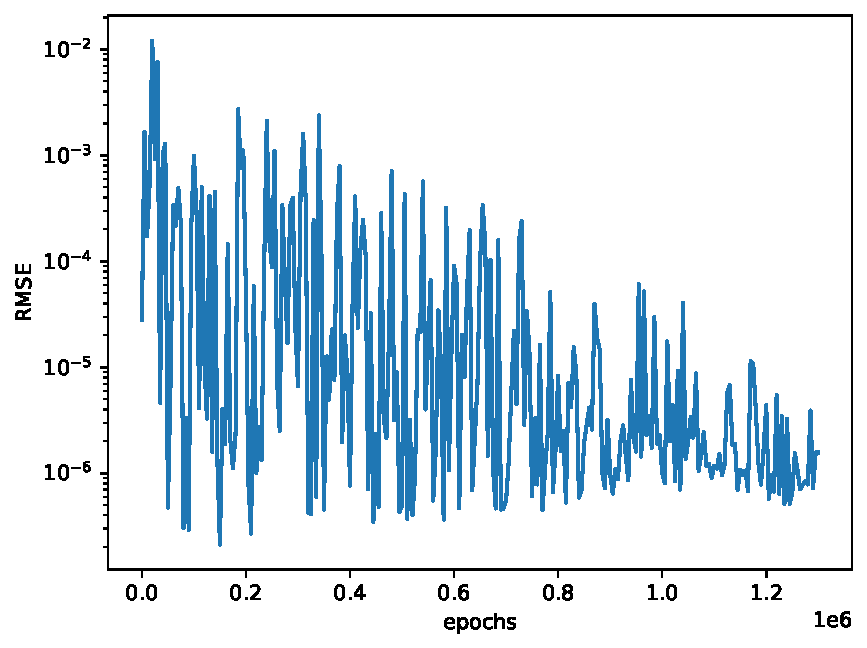
\includegraphics[width=0.42\linewidth]{ThesisFigs/bl_RMSE_001_96.pdf}}
\subfigure[\textit{bl}\label{update_bl_noinit96}]{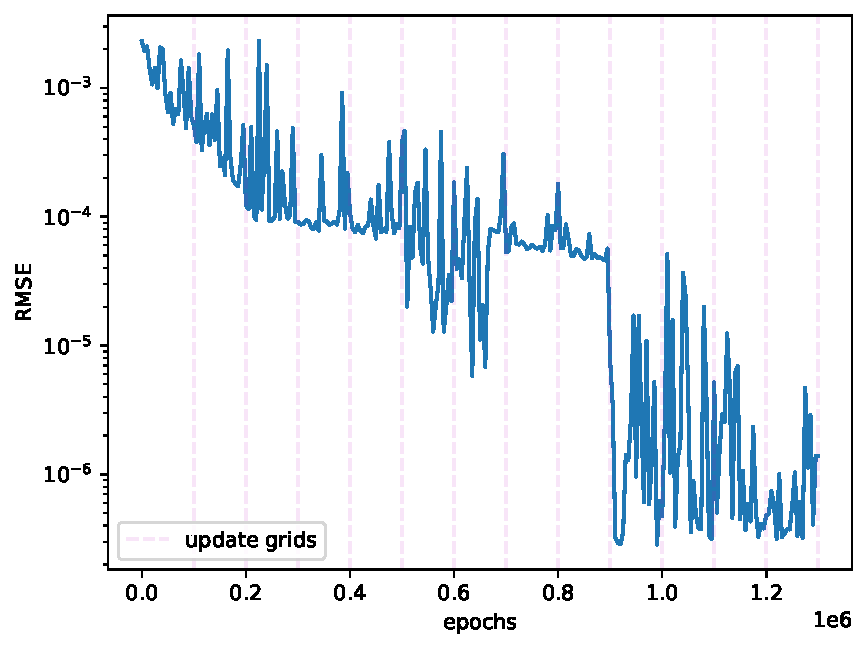
\includegraphics[width=0.42\linewidth]{ThesisFigs/bl_RMSE_010_96.pdf}}
\subfigure[\textit{spectral-basis}\label{update_sb_no96}]{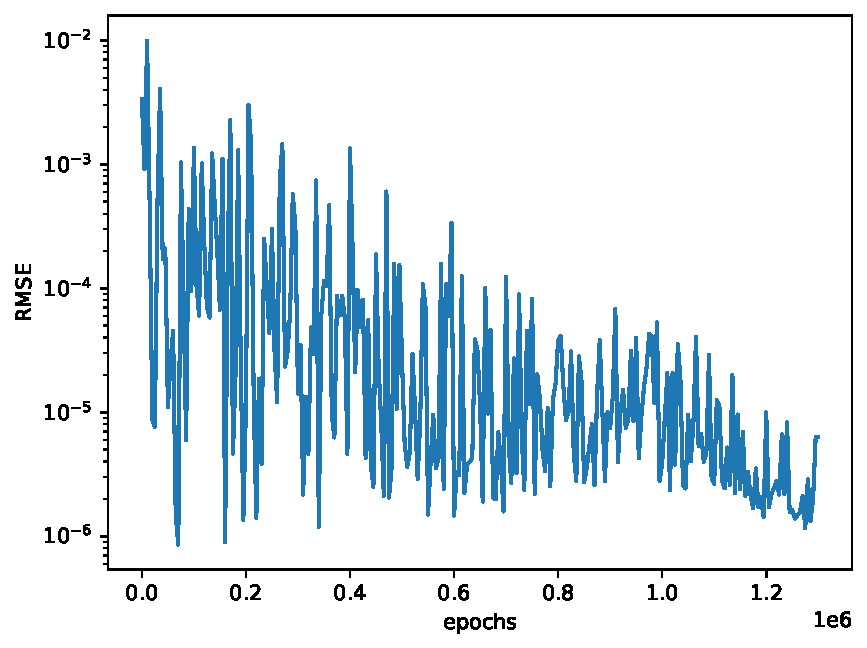
\includegraphics[width=0.42\linewidth]{ThesisFigs/sb_RMSE_001_96.pdf}}
\subfigure[\textit{spectral-basis}\label{update_sb_noinit96}]{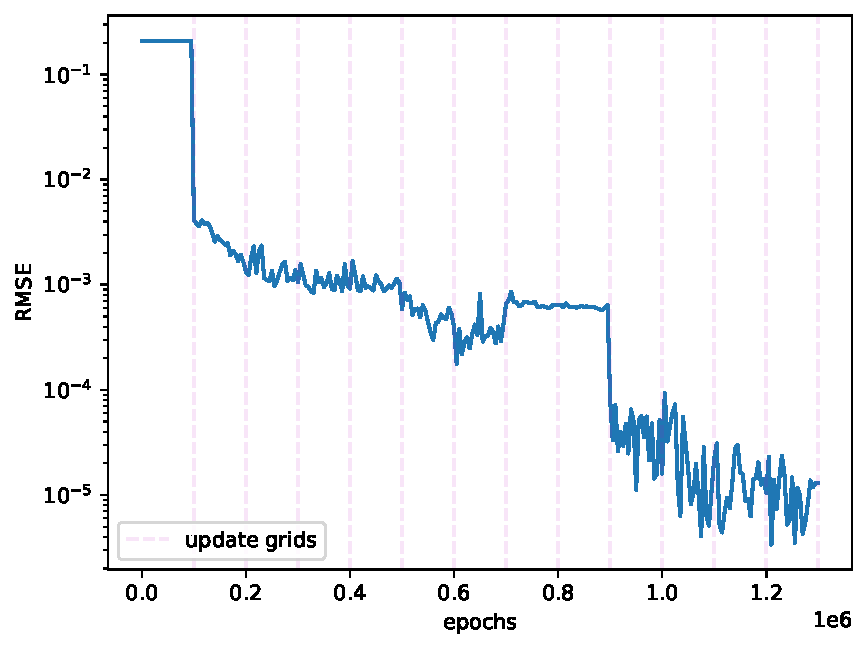
\includegraphics[width=0.42\linewidth]{ThesisFigs/sb_RMSE_010_96.pdf}}
\caption{For \textit{bl} and \textit{spectral-basis}, \cref{update_bl_no96} and \cref{update_sb_no96} correspondingly shows the RMSE for the constant degree $N_{degree}=96$; \cref{update_bl_noinit96} and \cref{update_sb_noinit96} correspondingly shows the RMSE for the variable degree}
\label{fig:update_96}
\end{figure}

\begin{table}[ht]
\caption{Computational cost for update of grids}
\label{table:cost for update}
\begin{center}
\begin{tabular}{lll}
% \multicolumn{1}{c}{\bf Type}  & \multicolumn{1}{c}{\bf Function}  & \multicolumn{1}{c}{\bf Training rate (iter/sec)} \\ 
\hline
constant degree & \textit{spectral-bias} & $7.82\times 10^2$ \\
variable degree & \textit{spectral-bias} & $7.82\times 10^2$ \\
constant degree & \textit{bl} & $7.67\times 10^2$ \\
variable degree & \textit{bl} & $7.73\times 10^2$ \\
\end{tabular}
\end{center}
\end{table}

\section{Results of selected $h$}\label{Appendix: select_h}
The comprehensive results of the selected ${h_i}$ parameters are presented in \cref{table: sin-low with inverse decay} and \cref{table: sin-low with exponential decay}. The complexity of parameter optimization increases substantially when $h_i$ assumes larger values. For instance, regarding large $h$ values on fine grids, it is hypothesized that $N_{degree}=100$ may not fully exploit the available capabilities. Consequently, an additional experimental investigation was conducted utilizing 5000 grid points, with ${h_i}={1/10,1/100,1/1000}$, and $N_{degree}=500$. The results demonstrated RMSE values of $7.92e\mbox{-}4\pm 4.21e\mbox{-}4$ for sin-low and $2.32e\mbox{-}3\pm 2.74e\mbox{-}4$ for sin-high. These findings indicate that enhanced accuracy can be achieved for sin-high through further hyperparameter optimization of the SincKAN model.
\begin{figure}[ht]%[H]%
\centering %%$u_t = \epsilon{\partial^6 u\over \partial x^6}$ %%$u_t = \epsilon{\partial^{10} u\over \partial x^{10}}$
\subfigure[\label{sin_low_inverse}]{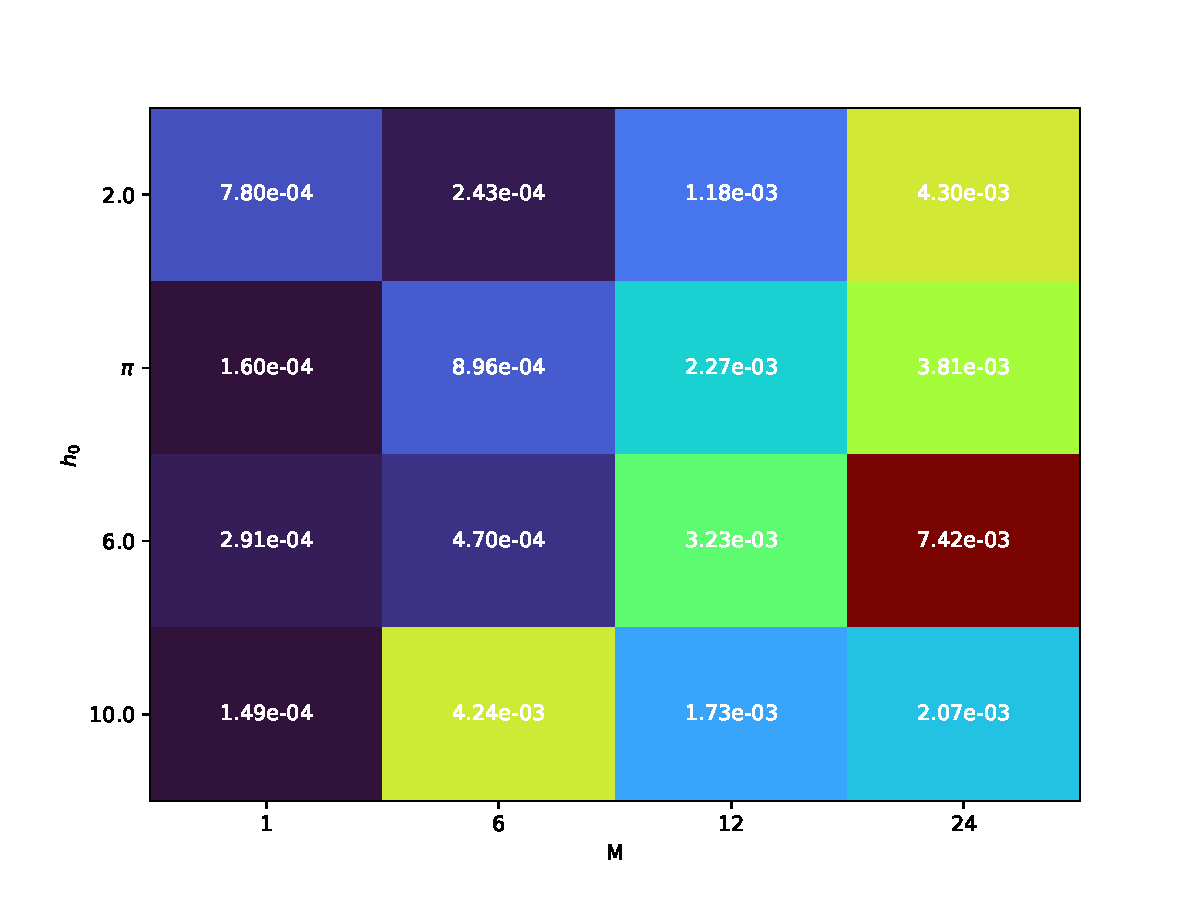
\includegraphics[width=0.4\linewidth]{ThesisFigs/sin_low_inverse.pdf}} %width==0.329
\subfigure[\label{sin_high_inverse}]{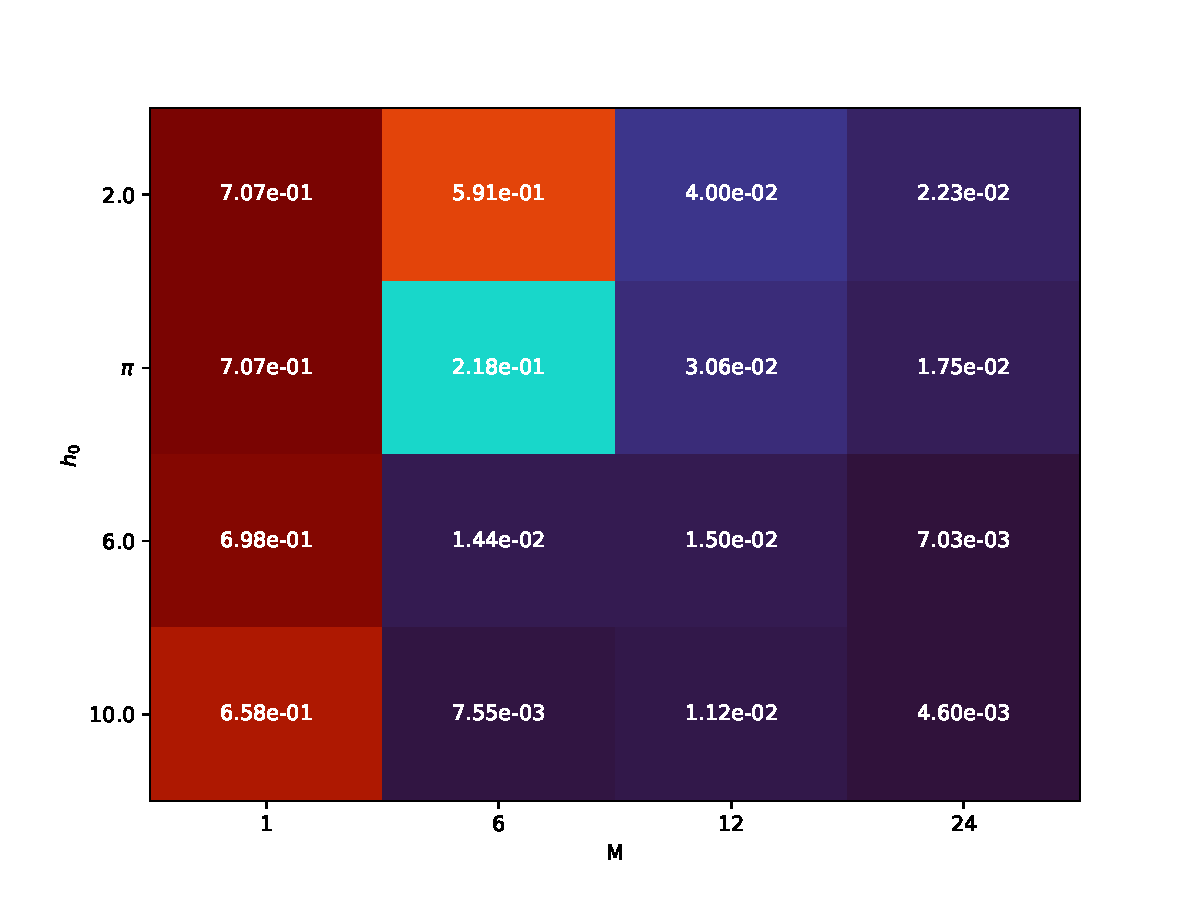
\includegraphics[width=0.4\linewidth]{ThesisFigs/sin_high_inverse.pdf}}
\caption{\cref{sin_low_inverse} shows the inverse decay approach on sin-low function; \cref{sin_high_inverse} shows the inverse decay approach on sin-high function.}
\label{fig:select_h_inverse}
\end{figure}
\begin{figure}[ht]%[H]%
\centering %%$u_t = \epsilon{\partial^6 u\over \partial x^6}$ %%$u_t = \epsilon{\partial^{10} u\over \partial x^{10}}$
\subfigure[\label{sin_low_exp}]{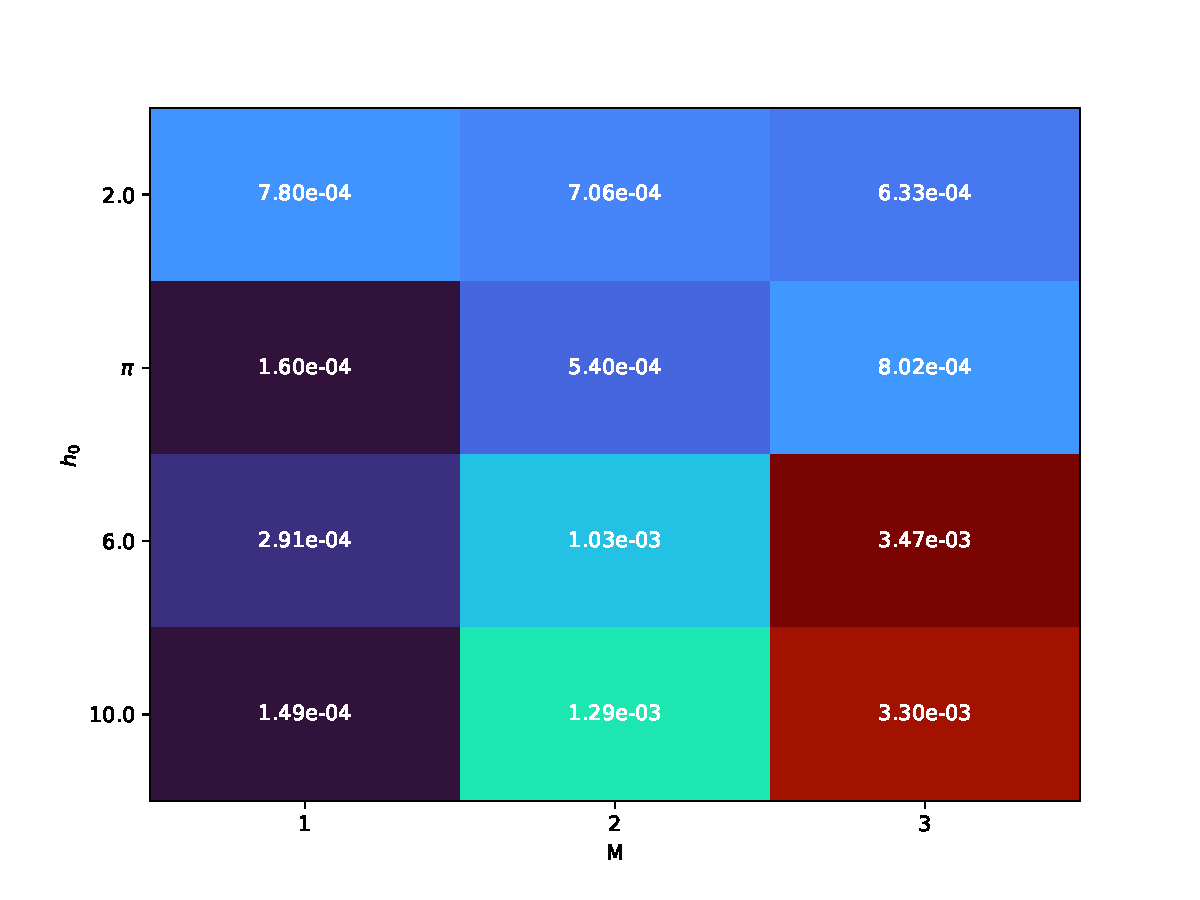
\includegraphics[width=0.4\linewidth]{ThesisFigs/sin_low_exp.pdf}}
\subfigure[\label{sin_high_exp}]{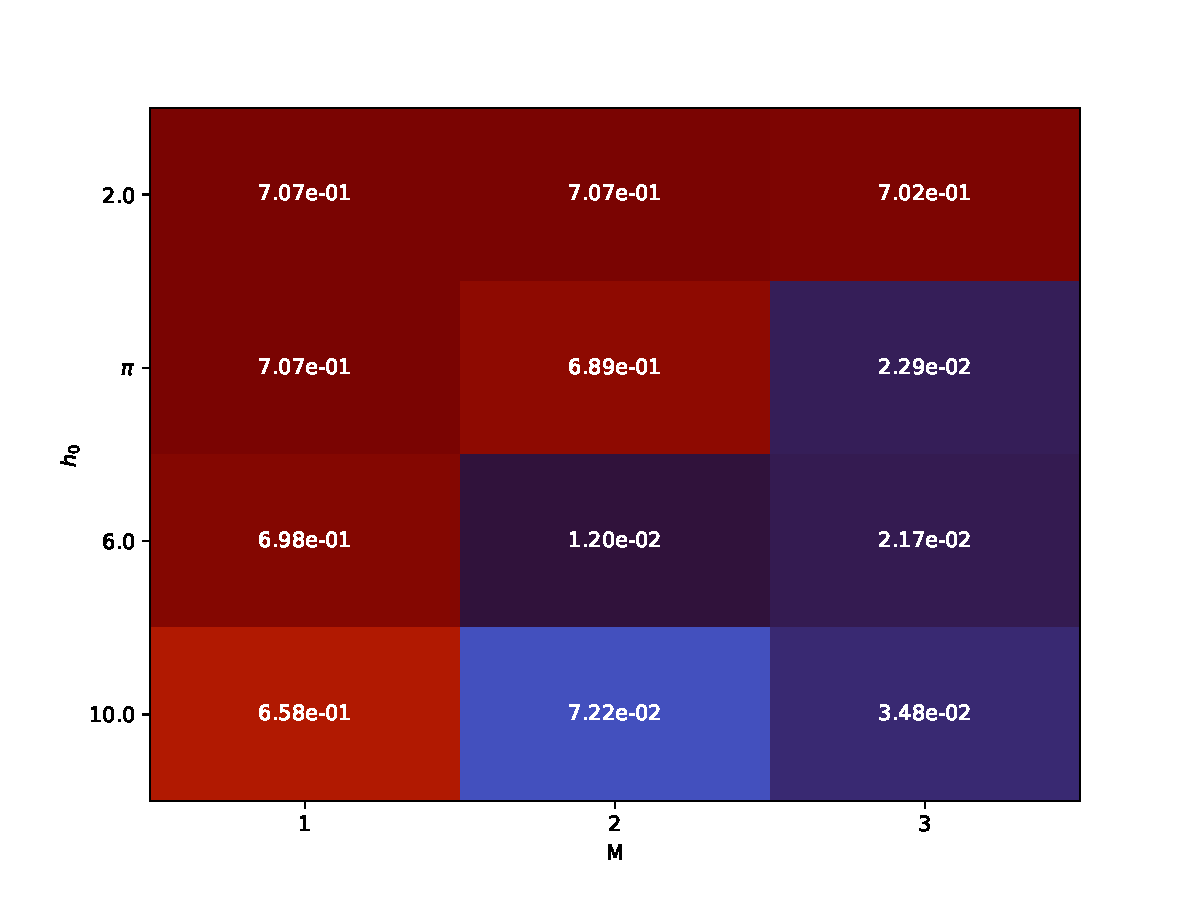
\includegraphics[width=0.4\linewidth]{ThesisFigs/sin_high_exp.pdf}}
\caption{\cref{sin_low_exp} shows the exponential decay approach on sin-low function; \cref{sin_high_exp} shows the exponential decay approach on sin-high function.}
\label{fig:select_h_exp}
\end{figure}
\begin{table}[ht]
\caption{RMSE for different $\{h_i\}$ with inverse decay}
\label{table: sin-low with inverse decay}
\begin{center}
\begin{adjustbox}{width=\columnwidth, center}
\begin{tabular}{llllll}
\multicolumn{1}{c}{\bf Function name}&$h_0$ $\setminus$ M& \multicolumn{1}{c}{1} &\multicolumn{1}{c}{6} & \multicolumn{1}{c}{12} & \multicolumn{1}{c}{24}
\\ \hline
\multirow{4}{*}{sin-low} &2.0     & $7.80e\mbox{-}4 \pm 7.96e\mbox{-}4$   & $2.43e\mbox{-}4 \pm 1.55e\mbox{-}4$ & $1.18e\mbox{-}3 \pm 2.38e\mbox{-}4$ & $4.30e\mbox{-}3 \pm 1.74e\mbox{-}3$ \\
                         & $\pi$  & $1.60e\mbox{-}4 \pm 6.66e\mbox{-}5$   & $8.96e\mbox{-}4 \pm 5.91e\mbox{-}4$ & $2.27e\mbox{-}3 \pm 8.53e\mbox{-}4$ & $3.81e\mbox{-}3 \pm 2.47e\mbox{-}3$ \\
                         & 6.0    & $2.91e\mbox{-}4 \pm 1.22e\mbox{-}4$   & $4.70e\mbox{-}4 \pm 1.88e\mbox{-}4$ & $3.23e\mbox{-}3 \pm 8.47e\mbox{-}4$ & $7.42e\mbox{-}3 \pm 7.40e\mbox{-}3$ \\
                         & 10.0   & \color{red}{$1.49e\mbox{-}4 \pm 8.74e\mbox{-}5$}   & $4.24e\mbox{-}3 \pm 3.18e\mbox{-}3$ & $1.73e\mbox{-}3 \pm 1.08e\mbox{-}3$ & $2.07e\mbox{-}3 \pm 8.84e\mbox{-}4$ \\
\\
\multirow{4}{*}{sin-high}&2.0     & $7.07e\mbox{-}1 \pm 6.70e\mbox{-}6$  & $5.91e\mbox{-}1 \pm 6.32e\mbox{-}3$ & $4.00e\mbox{-}2 \pm 1.24e\mbox{-}3$ & $2.23e\mbox{-}2 \pm 1.38e\mbox{-}3$  \\ 
                         & $\pi$  &  $7.07e\mbox{-}1 \pm 7.94e\mbox{-}6$ & $2.18e\mbox{-}1 \pm 1.88e\mbox{-}2$ & $3.06e\mbox{-}2 \pm 2.80e\mbox{-}3$ & $1.75e\mbox{-}2 \pm 2.44e\mbox{-}3$  \\ 
                         & 6.0    & $6.98e\mbox{-}1 \pm 4.88e\mbox{-}3$  & $1.44e\mbox{-}2 \pm 1.34e\mbox{-}3$ & $1.50e\mbox{-}2 \pm 8.68e\mbox{-}4$ & $7.03e\mbox{-}3 \pm 1.95e\mbox{-}3$  \\ 
                         & 10.0   & $6.58e\mbox{-}1 \pm 3.32e\mbox{-}3$  & $7.55e\mbox{-}3 \pm 1.73e\mbox{-}3$ & $1.12e\mbox{-}2 \pm 2.75e\mbox{-}3$ & \color{red}{$4.60e\mbox{-}3 \pm 3.70e\mbox{-}4$}  \\ 
\end{tabular}
\end{adjustbox}
\end{center}
\end{table}
\begin{table}[ht]
\caption{RMSE for different $\{h_i\}$ with exponential decay}
\label{table: sin-low with exponential decay}
\begin{center}
\begin{adjustbox}{width=\columnwidth, center}
\begin{tabular}{lllll}
\multicolumn{1}{c}{\bf Function name}& $h_0$ $\setminus$ M& \multicolumn{1}{c}{1} &\multicolumn{1}{c}{2} & \multicolumn{1}{c}{3}
\\ \hline 
\multirow{4}{*}{sin-low} &2.0     & $7.80e\mbox{-}4 \pm 7.96e\mbox{-}4$   & $7.06e\mbox{-}4 \pm 2.54e\mbox{-}4$ & $6.33e\mbox{-}4 \pm 1.38e\mbox{-}4$  \\
                         & $\pi$  & $1.60e\mbox{-}4 \pm 6.66e\mbox{-}5$   & $5.40e\mbox{-}4 \pm 2.05e\mbox{-}4$ & $8.02e\mbox{-}4 \pm 6.58e\mbox{-}5$  \\
                         & 6.0    & $2.91e\mbox{-}4 \pm 1.22e\mbox{-}4$   & $1.03e\mbox{-}3 \pm 3.78e\mbox{-}4$ & $3.47e\mbox{-}3 \pm 3.31e\mbox{-}4$  \\
                         & 10.0   & \color{red}{$1.49e\mbox{-}4 \pm 8.74e\mbox{-}5$}   & $1.29e\mbox{-}3 \pm 1.74e\mbox{-}4$ & $3.30e\mbox{-}3 \pm 2.80e\mbox{-}4$  \\
\\
\multirow{4}{*}{sin-high} &2.0     & $7.07e\mbox{-}1 \pm 6.70e\mbox{-}6$    & $7.07e\mbox{-}1 \pm 1.42e\mbox{-}5$ & $7.02e\mbox{-}1 \pm 2.84e\mbox{-}3$ \\
                         & $\pi$  & $7.07e\mbox{-}1 \pm 7.94e\mbox{-}6$    & $6.89e\mbox{-}1 \pm 4.82e\mbox{-}3$ & $2.29e\mbox{-}2 \pm 1.76e\mbox{-}3$ \\
                         & 6.0    & $6.98e\mbox{-}1 \pm 4.88e\mbox{-}3$    & \color{red}{$1.20e\mbox{-}2 \pm 1.35e\mbox{-}3$} & $2.17e\mbox{-}2 \pm 6.67e\mbox{-}4$ \\
                         & 10.0   & $6.58e\mbox{-}1 \pm 3.32e\mbox{-}3$    & $7.22e\mbox{-}2 \pm 8.12e\mbox{-}3$ & $3.48e\mbox{-}2 \pm 2.38e\mbox{-}3$ \\
\end{tabular}
\end{adjustbox}
\end{center}
\end{table}
\section{Oscillations of SincKAN} \label{Appendix: oscillation}
Experimental investigations were conducted on convection-diffusion equations (\cref{eq:cd}) utilizing various parameter combinations: $h_0=2.0,10.0$, $N=8,100$, and $M=1,6$. With the exception of the configuration where $h_0=2.0$ and $N=8$, derivative inaccuracies resulted in SincKAN instability, manifesting as divergent loss patterns. Selected visualizations in \cref{fig:oscillation} demonstrate the oscillatory behavior that constrains SincKAN performance enhancement.
\begin{figure}[ht]%[H]%
\centering %%$u_t = \epsilon{\partial^6 u\over \partial x^6}$ %%$u_t = \epsilon{\partial^{10} u\over \partial x^{10}}$
\subfigure[\label{2_8_1} $h_0=2.0, N=8, M=1$]{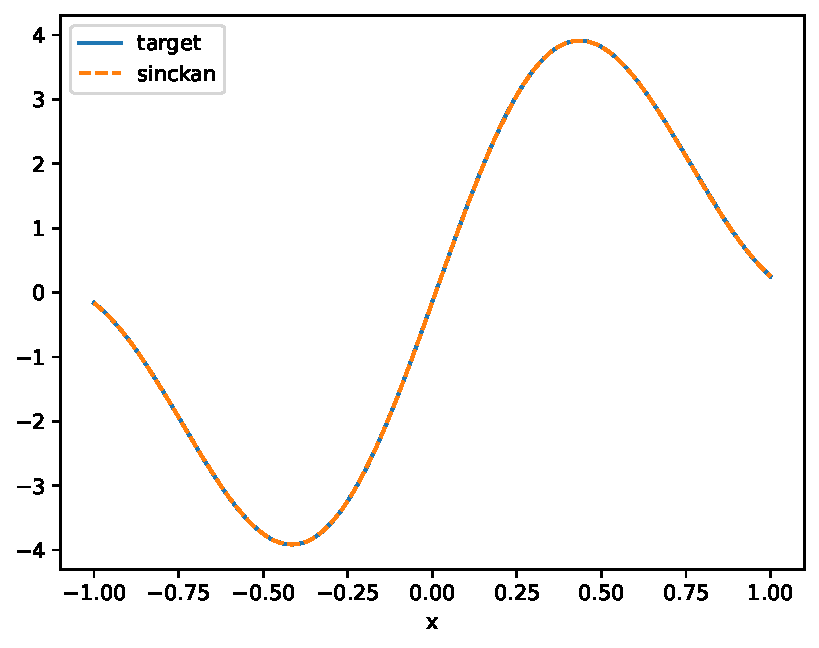
\includegraphics[width=0.4\linewidth]{ThesisFigs/cd_2_8_1.pdf}} %width==0.329
\subfigure[\label{2_8_6} $h_0=2.0, N=8, M=6$]{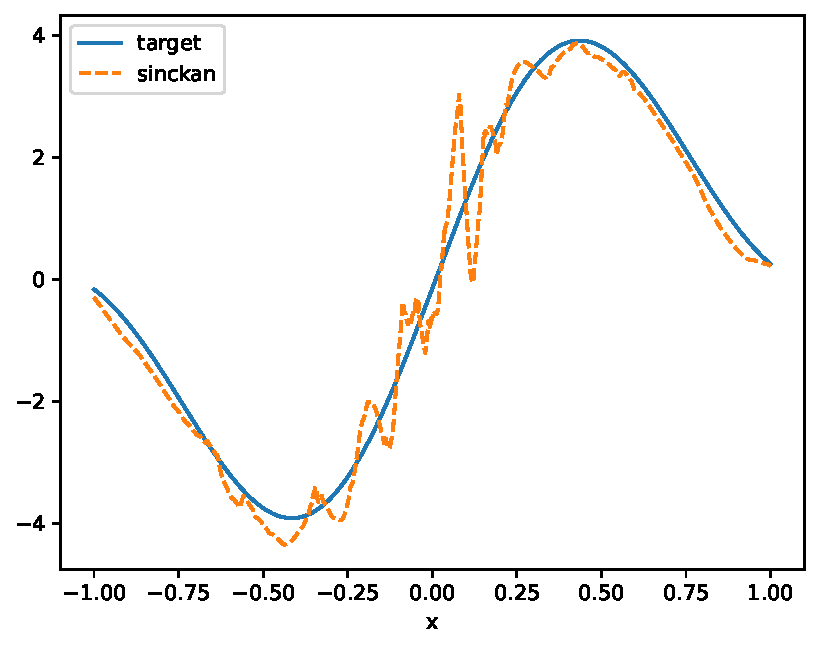
\includegraphics[width=0.4\linewidth]{ThesisFigs/cd_2_8_6.pdf}}
\subfigure[\label{10_8_1} $h_0=10.0, N=8, M=1$]{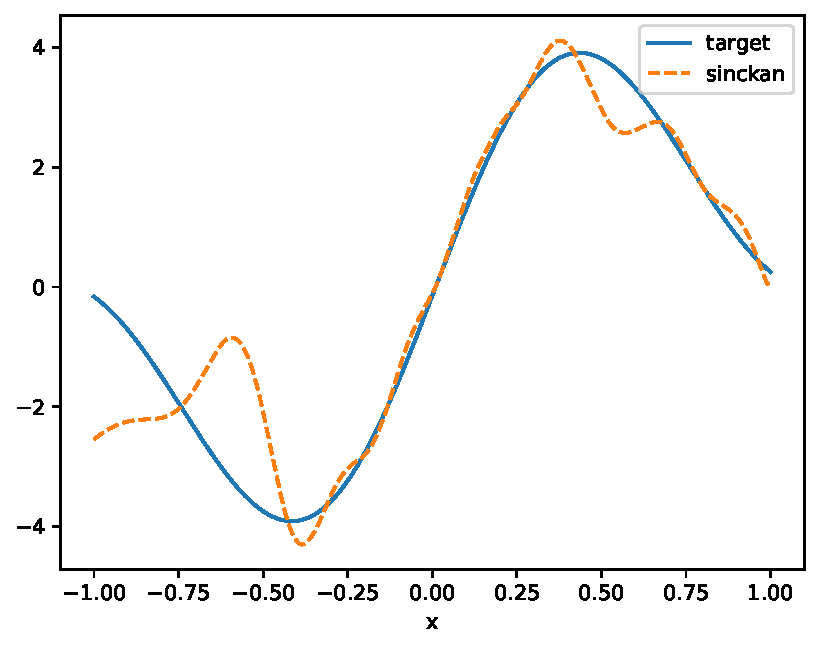
\includegraphics[width=0.4\linewidth]{ThesisFigs/cd_10_8_1.pdf}}
\subfigure[\label{2_100_6} $h_0=2.0, N=100, M=6$]{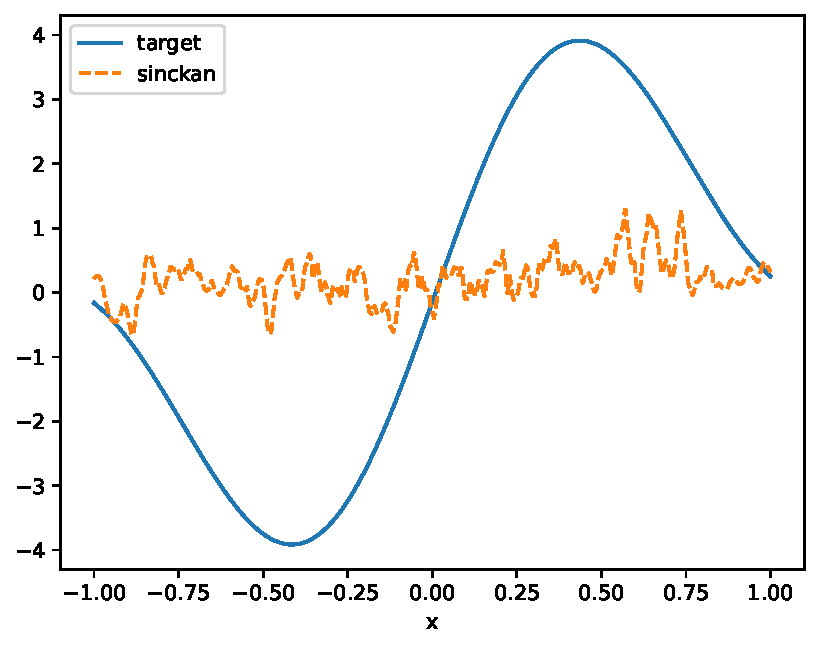
\includegraphics[width=0.4\linewidth]{ThesisFigs/cd_2_100_6.pdf}}
\caption{\cref{2_8_1} solve \cref{eq:cd} accurately. However, SincKANs have oscillations after either increasing $M$ (\cref{2_8_6}) or increasing $h_0$. \cref{2_100_6} shows that with the same hyperparameters used in approximation, SincKAN becomes extremely inaccurate due to the violent oscillations.}
\label{fig:oscillation}
\end{figure}
\section{Metrics}
In this research, two primary metrics were employed. For interpolation purposes, the RMSE metric was adopted from KAN~\cite{liu2024kan}, defined as:
\begin{equation}
\mathrm{RMSE}=\sqrt{\frac{1}{N}\sum_{i=1}^{N}(y_i-\hat{y}_i)^2};
\end{equation}
For PIKANs, the relative L2 error, commonly utilized in PINNs, was implemented:
\begin{equation}
    \mathrm{Relative L2}=\frac{\|\boldsymbol{y}-\hat{\boldsymbol{y}}\|_2}{\|\boldsymbol{y}\|_2},
\end{equation}
where $y$ represents the target value and $\hat{y}$ denotes the predicted value.

% ------------------------------------------------------------------------

%%% Local Variables: 
%%% mode: latex
%%% TeX-master: "../thesis"
%%% End: 
